\documentclass[manuscript,screen,review]{jair}
% Submission-stage metadata controls: suppress sample rights/DOI/editor blocks.
\setcopyright{none}
\acmDOI{}
\JAIRAE{}
\JAIRTrack{}
\makeatletter
\def\@mkbibcitation{}
\let\footnotetextcopyrightpermission\@gobble
\makeatother

\RequirePackage[
  datamodel=acmdatamodel,
  style=acmauthoryear,
  backend=biber,
  giveninits=true,
  uniquename=init
]{biblatex}
\addbibresource{references.bib}
\renewcommand*{\bibopenbracket}{(}
\renewcommand*{\bibclosebracket}{)}

\usepackage{booktabs,graphicx,microtype,tabularx,array,tikz}
\usepackage{xcolor}
\usetikzlibrary{arrows.meta,positioning,fit,calc,shapes.geometric}
\newcolumntype{Y}{>{\raggedright\arraybackslash}X}

\newtheorem{theorem}{Theorem}
\newtheorem{proposition}[theorem]{Proposition}
\newtheorem{corollary}[theorem]{Corollary}
\newcommand{\Prb}{\mathbb{P}}
\newcommand{\E}{\mathbb{E}}
\newcommand{\ind}{\mathbf{1}}

\title[Fairness After the Decision]{Fairness After the Decision: Group Fairness Under Selective Human Contestation}
\author{Ranjan Veerabhadraswamy}
\affiliation{%
  \department{School of Computer Science and Engineering}
  \institution{Vellore Institute of Technology, Andhra Pradesh}
  \city{Amaravati, Andhra Pradesh 522241}
  \country{India}}
\email{ranjanvswamyjnv2005@gmail.com}

\author{Ajith Jubilson Emerson}
\authornote{Corresponding author.}
\affiliation{%
  \department{School of Computer Science and Engineering}
  \institution{Vellore Institute of Technology, Andhra Pradesh}
  \city{Amaravati, Andhra Pradesh 522241}
  \country{India}}
\email{ajith.jubilson@vitap.ac.in}
\renewcommand{\shortauthors}{Veerabhadraswamy and Emerson}
\hypersetup{
  pdftitle={Fairness After the Decision: Group Fairness Under Selective Human Contestation},
  pdfauthor={Ranjan Veerabhadraswamy and Ajith Jubilson Emerson},
  pdfcopyright={},
  pdflicenseurl={}}

\begin{document}

\begin{abstract}
{\bf Background:} Group-fairness analyses often stop at an algorithm's initial
decision even when affected people may enter a selective human review process.
{\bf Objectives:} We characterize how claimant-initiated contestation changes
standard group-fairness quantities and what ordinary appeal logs identify.
{\bf Methods:} A label- and group-specific post-decision operator separates
appeal access from review quality.  We derive exact preservation and signed-gap
conditions, analyze heterogeneous-cost access and budgeted assistance, and
obtain appeal-log-specific sharp bounds.  Synthetic checks and 600 paired
semisynthetic Adult/German Credit runs evaluate the formal predictions.
{\bf Results:} Adult supports signed movement and absolute equal-opportunity-gap
amplification in all 12 unequal-access model--scenario cells.  On German
Credit, the predicted signed direction is statistically resolved in 7 of 12
cells, including none of the four random-forest cells; no cell supports broad
absolute-gap amplification.
{\bf Conclusions:} Selective review can create, reinforce, attenuate, cross, or
reverse disparity.  Empirical validation is partial rather than universal,
and auditing must cover the initial decision, access, review, and final action.

\begin{center}
\centering
\resizebox{.95\linewidth}{!}{%
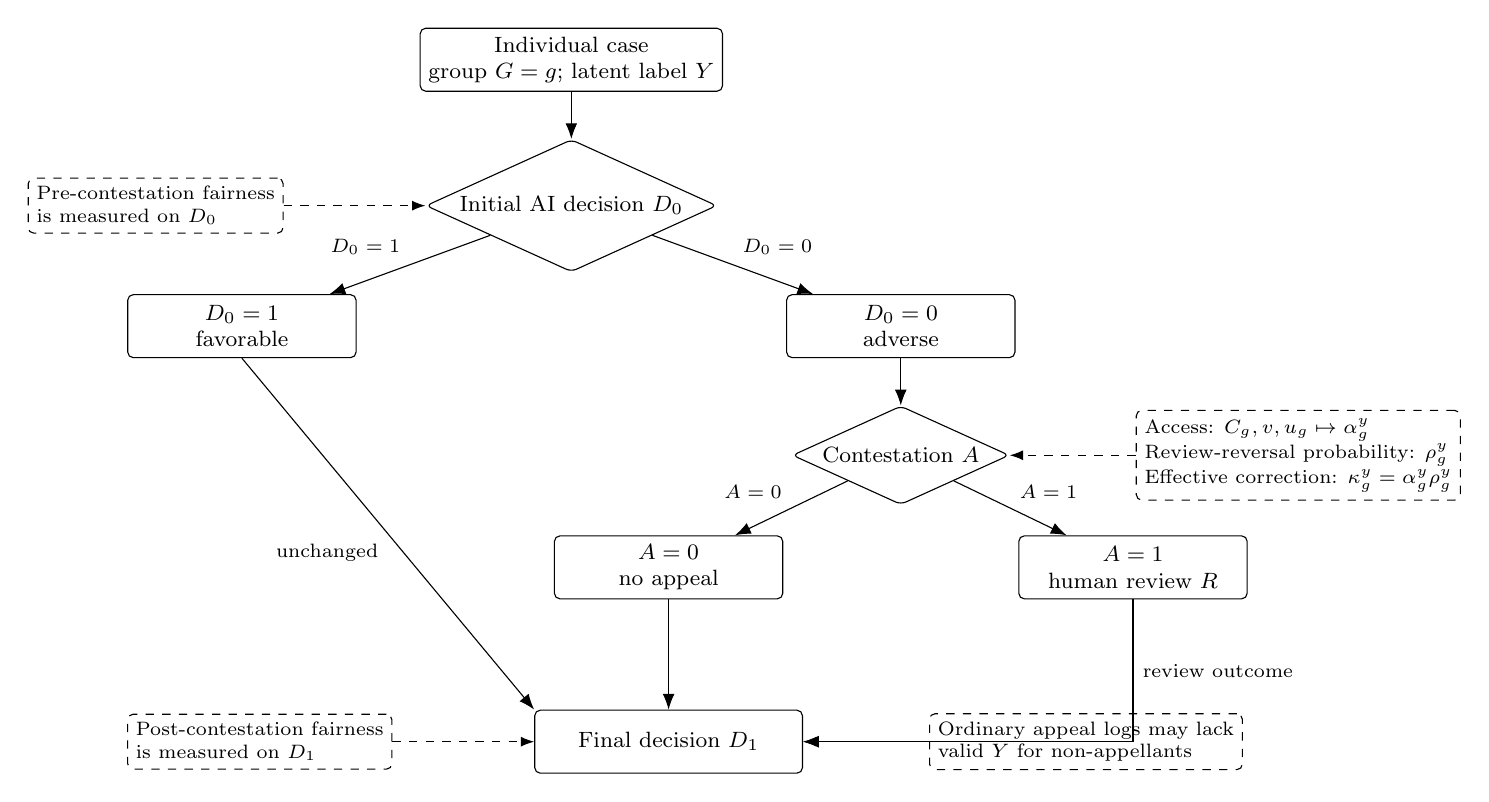
\begin{tikzpicture}[
  font=\footnotesize,
  node distance=6mm and 13mm,
  box/.style={draw,rounded corners=2pt,align=center,inner sep=3pt,
    minimum height=8mm,minimum width=29mm,fill=white},
  choice/.style={box,diamond,aspect=2.2,inner sep=1.5pt,minimum width=24mm},
  note/.style={draw,dashed,rounded corners=2pt,align=left,inner sep=3pt,
    font=\scriptsize},
  flow/.style={-{Latex[length=2mm]},thin},
  link/.style={-{Latex[length=1.7mm]},thin,dashed}
]
\node[box] (case) {Individual case\\group $G=g$; latent label $Y$};
\node[choice,below=of case] (d0) {Initial AI decision $D_0$};
\node[box,below left=7mm and 18mm of d0] (fav) {$D_0=1$\\favorable};
\node[box,below right=7mm and 18mm of d0] (adv) {$D_0=0$\\adverse};
\node[choice,below=of adv] (appeal) {Contestation $A$};
\node[box,below left=7mm and 8mm of appeal] (noapp) {$A=0$\\no appeal};
\node[box,below right=7mm and 8mm of appeal] (review) {$A=1$\\human review $R$};
\node[box,below=14mm of noapp,minimum width=34mm] (d1) {Final decision $D_1$};
\draw[flow] (case) -- (d0);
\draw[flow] (d0) -- node[above left,font=\scriptsize] {$D_0=1$} (fav);
\draw[flow] (d0) -- node[above right,font=\scriptsize] {$D_0=0$} (adv);
\draw[flow] (adv) -- (appeal);
\draw[flow] (appeal) -- node[above left,font=\scriptsize] {$A=0$} (noapp);
\draw[flow] (appeal) -- node[above right,font=\scriptsize] {$A=1$} (review);
\draw[flow] (fav.south) -- node[below left,font=\scriptsize] {unchanged} (d1.north west);
\draw[flow] (noapp) -- (d1);
\draw[flow] (review.south) |- node[pos=.25,right,font=\scriptsize]
  {review outcome} (d1.east);

\node[note,left=18mm of d0] (pre) {Pre-contestation fairness\\is measured on $D_0$};
\node[note,left=18mm of d1] (post) {Post-contestation fairness\\is measured on $D_1$};
\draw[link] (pre.east) -- (d0.west);
\draw[link] (post.east) -- (d1.west);
\node[note,right=16mm of appeal] (access)
  {Access: $C_g,v,u_g\mapsto\alpha_g^y$\\Review-reversal probability: $\rho_g^y$\\
   Effective correction: $\kappa_g^y=\alpha_g^y\rho_g^y$};
\draw[link] (access.west) -- (appeal.east);
\node[note,right=16mm of d1] (logs)
  {Ordinary appeal logs may lack\\valid $Y$ for non-appellants};
\draw[link] (logs.west) -- (d1.east);
\end{tikzpicture}}
\captionof{figure}{The post-decision Human--AI contestation mechanism.  An adverse
initial AI decision may enter a self-selected appeal channel; human review may
reverse the decision.  Group- and label-specific appeal access $\alpha_g^y$
and review-reversal probability $\rho_g^y$ determine effective transition probabilities
$\kappa_g^y$, so fairness of $D_0$ need not equal fairness of $D_1$.  The
label $Y$ is a latent ground-truth quantity used for analysis, not information
assumed available at decision time.}
\Description{A process diagram from an individual case through the initial AI
decision. Favorable decisions proceed directly to the final decision; adverse
decisions may enter selective contestation and human review before the final
decision. Side notes identify access, review-reversal probability, fairness measurement,
and missing labels in ordinary appeal logs.}
\label{fig:architecture}
\end{center}
\end{abstract}

\maketitle
\hypersetup{
  pdfauthor={Ranjan Veerabhadraswamy and Ajith Jubilson Emerson},
  pdfcopyright={},
  pdflicenseurl={}}

\section{Introduction}

A denied loan, benefit, job, or service is not always the final institutional
action.  A person may submit evidence, navigate an appeal process, or obtain
human review.  Entry into that process is rarely random: time, information,
documentation, language, legal help, and expected benefit all affect who
contests.  Consequently, two groups can face the same formal appeal rule but
different effective opportunities to correct an error.

This observation creates a distinct fairness problem.  Classifier metrics
describe the initial decision, whereas people experience the final decision
after review.  A correction channel can improve aggregate accuracy while
redistributing that improvement unequally.  Conversely, differential review
can sometimes reduce an existing absolute disparity.  The relevant object is thus not an
informal ``right to appeal,'' but a stochastic post-decision transformation
whose transition probabilities depend on group, latent label, initial outcome,
and policy.

We study a binary, one-shot model in which an individual with an adverse
initial decision may appeal and review may reverse that decision.  Let
$\alpha_g^+$ be the probability that a false denial in group $g$ is appealed
and $\rho_g^+$ its conditional correction probability; let $\alpha_g^-$ and
$\rho_g^-$ analogously describe an appealed correct denial that is incorrectly
reversed.  The effective transition rates are
$\kappa_g^+=\alpha_g^+\rho_g^+$ and
$\kappa_g^-=\alpha_g^-\rho_g^-$.  This factorization separates access from
review quality while making clear that final fairness depends on their product.

Our contributions are deliberately narrow: (i) exact fairness transformation
and preservation characterization for a post-decision contestation operator;
(ii) signed disparity dynamics, including creation, amplification,
attenuation, crossing, and reversal; (iii) group-fairness consequences of
endogenous participation under heterogeneous costs and formally symmetric
policies; (iv) appeal-log-specific non-identification and sharp final-FNR and
disparity bounds; and (v) resource-constrained assistance within the same
mechanism.  We do not claim generic novelty for contestability, procedural
fairness, recourse burdens or costs, selective labels, partial identification,
random auditing, convex optimization, or knapsack structure.

The empirical evidence is intentionally qualified.  Synthetic experiments
verify the formal results.  Semisynthetic experiments use real prediction
tasks but simulated contestation, not observed human appeals.  Adult
consistently exhibits the predicted signed shifts and absolute-gap increases,
whereas German Credit provides partial directional support and no model-robust
evidence of absolute-gap amplification.
Figure~\ref{fig:architecture} summarizes the mechanism and the distinction
between pre- and post-contestation fairness.

\begin{table}[t]
\centering
\caption{Notation and acronyms used throughout the paper.}
\label{tab:notation}
\footnotesize
\begin{tabularx}{\linewidth}{@{}>{\raggedright\arraybackslash}p{.19\linewidth}Y
  >{\raggedright\arraybackslash}p{.30\linewidth}@{}}
\toprule
Symbol/acronym & Meaning & Definition/domain \\
\midrule
$G,g$ & Protected-group variable and a group & $G\in\mathcal G$ \\
$Y$ & Latent target/ground-truth label & $\{0,1\}$; not assumed observed at decision time \\
$D_0,D_1$ & Initial and final decisions & $\{0,1\}$; 0 is adverse \\
$A,R$ & Appeal indicator; review reversal indicator & $\{0,1\}$ \\
$t_g,f_g$ & Initial true- and false-positive rates & $\Prb(D_0=1\mid Y=1,g)$; $\Prb(D_0=1\mid Y=0,g)$ \\
TPR/FNR & True-positive / false-negative rates & $\mathrm{TPR}_g=t_g$; $\mathrm{FNR}_g=1-t_g$ \\
FPR/TNR & False-positive / true-negative rates & $\mathrm{FPR}_g=f_g$; $\mathrm{TNR}_g=1-f_g$ \\
$\pi_g$ & Positive-label prevalence & $\Prb(Y=1\mid G=g)$ \\
$\alpha_g^y,\rho_g^y$ & Appeal access; conditional review-reversal probability & Conditional probabilities in $[0,1]$ \\
$\kappa_g^y$ & Effective correction transition & $\alpha_g^y\rho_g^y$ \\
$\Delta_{EO},\Delta_{FPR}$ & Signed EO and FPR disparities & Group-$a$ rate minus group-$b$ rate \\
$C_g,v,u_g$ & Appeal cost, perceived benefit, group assistance & $\alpha_g(u_g)=F_g(v+u_g)$ \\
$B,N_g$ & Assistance budget; eligible group population & $\sum_g N_gu_g\le B$ \\
$\mathcal R_g(u_g)$ & Group residual false-negative risk & $\mathrm{FNR}_g[1-\rho_g^+\alpha_g^+(u_g)]$ \\
$d_g,a_g,\eta_g,q_g$ & Adverse mass, appeal rate, appellant positive-label share, non-appellant positive-label share & Probabilities in $[0,1]$ \\
$s_g,m_g,n_g$ & Favorable-positive, appealed-positive, and adverse-non-appellant masses & Nonnegative observed masses in the bounds \\
$\epsilon,\lambda$ & Residual-risk target; fairness-penalty weight & Nonnegative policy parameters \\
$K_g^y,T_K,L$ & Label-specific transition kernel, induced linear operator, fairness map & Stochastic/linear operators \\
EO/DP & Equal opportunity; demographic parity & Group-fairness criteria \\
KKT/IPW & Karush--Kuhn--Tucker; inverse-probability weighting & Optimization/estimation tools \\
\bottomrule
\end{tabularx}
\end{table}

\section{Related work and positioning}

Contestability and correctability research motivates rights, evidence, and
infrastructure for challenging automated decisions
\citep{kaminski2021,cobbe2021,lyons2021,lyons2022,freiesleben2026}.  Perdana's
``correctability gap'' is a useful motivation: conventional fairness metrics
do not show whether affected people can appeal, submit evidence, or obtain
human review \citep{perdana2026legitimacy}.  We formalize one such correction
channel rather than treating correctability itself as new.

Procedural fairness studies the fairness of the decision-making process.
Wang et al. formalize individual and group procedural fairness using
feature-attribution characterizations of the model process
\citep{wang2026procedural}.  Our object begins after the model has issued
$D_0$: self-selected access to human review and the resulting $D_1$.
Relatedly, human discretion can change fairness in machine-assisted decisions
\citep{gillis2022,angelova2023}; here review is claimant-initiated rather than
discretion applied across all cases.

Differential parity compares two sets of decisions and asks whether their
difference is independent of a sensitive attribute, including human and model
comparisons and bridge estimation across different data
\citep{yu2026differential}.  We do not propose another relative-fairness
metric.  We specify the transition $D_0\to$ appeal $\to$ human review
$\to D_1$, make participation endogenous, and derive its transformation of
standard fairness quantities, identification properties, and interventions.

Recourse work shows that feasible actions, costs, and effectiveness vary
across groups \citep{vonkugelgen2020,kavouras2023}.  Nitchals separately
analyzes heterogeneous private appeal costs, procedural pricing, correction,
resource use, deterrence, and an interior optimal price
\citep{nitchals2026pricing}.  We make no novelty claim for heterogeneous costs
or resource-aware procedure design.  Our focus is protected-group fairness,
preservation of standard criteria, effective group-specific correction,
appeal-log identification, and fairness-aware assistance.

Selective-label research studies learning and fairness when outcomes are
observed only for selected cases
\citep{dearteaga2018,kilbertus2020,wei2021,coston2021,chen2025}.  Valdrighi et
al. address long-term fairness with selectively observed labels and sequential
policies \citep{valdrighi2026longterm}; Liu et al. study identification and
inference for fairness--accuracy frontiers \citep{liu2026frontiers}.  We do not
claim generic partial-identification novelty.  Our missingness comes from
self-selection into a post-decision correction channel, and we derive
appeal-specific sharp bounds for final FNR and associated group disparity.

Thus existing work separately studies contestability, procedural fairness,
relative decision-set fairness, human discretion, recourse burdens, appeal
economics, and selective-label identification.  We instead fix a specific
mechanism---an adverse AI decision may enter a self-selected human correction
channel---and ask how it transforms standard group-fairness properties and
what ordinary appeal records identify.

\begin{table}[t]
\centering
\caption{Positioning relative to closely related work.  The distinctions
summarize primary objects of analysis rather than asserting that a cited work
excludes every adjacent topic.}
\label{tab:related}
\footnotesize
\begin{tabularx}{\linewidth}{@{}p{.19\linewidth}p{.20\linewidth}p{.23\linewidth}Y@{}}
\toprule
Work & Primary focus & Review or identification setting & Relation to this work \\
\midrule
\citet{cobbe2021} & Reviewable automated decision-making & Institutional reviewability and contestability & Motivates review infrastructure; we formalize one transition mechanism. \\
\citet{gillis2022} & Machine-assisted human decisions & Human discretion across decisions & Our review is claimant-initiated after $D_0$. \\
\citet{wang2026procedural} & Procedural fairness of model decisions & Feature-attribution process criteria & Our object begins after $D_0$ and ends at $D_1$. \\
\citet{yu2026differential} & Relative fairness between decision sets & Differential parity and bridge estimation & We specify the mechanism producing $D_1$ and transform standard metrics. \\
\citet{freiesleben2026} & Contestability and recourse & Conceptual comparison of mechanisms & We analyze a particular claimant-initiated correction channel. \\
\citet{nitchals2026pricing} & Appeal costs and procedural pricing & Self-selected appeals; correction and deterrence & We focus on protected-group fairness, identification, and assistance. \\
\citet{valdrighi2026longterm}; \citet{liu2026frontiers} & Selective labels and fairness & Long-term fairness; frontier identification & Our missingness arises from self-selection into post-decision correction. \\
\bottomrule
\end{tabularx}
\end{table}

\section{Model}

Let $G\in\mathcal G$ denote group membership, $Y\in\{0,1\}$ the target label,
$D_0\in\{0,1\}$ the initial decision, and $D_1\in\{0,1\}$ the final decision.
Decision 0 is adverse.  Write
\[
 t_g=\Prb(D_0=1\mid Y=1,G=g),\qquad
 f_g=\Prb(D_0=1\mid Y=0,G=g),
\]
with $\mathrm{FNR}_g=1-t_g$ and $\mathrm{TNR}_g=1-f_g$.
Let $A$ indicate appeal and $R$ indicate reversal after review.  In the core
one-sided model, only $D_0=0$ cases can transition to $D_1=1$.  Define
\[
 \alpha_g^y=\Prb(A=1\mid D_0=0,Y=y,G=g),\quad
 \rho_g^y=\Prb(R=1\mid A=1,D_0=0,Y=y,G=g),
\]
and $\kappa_g^y=\alpha_g^y\rho_g^y$.  The superscripts $+$ and $-$ refer to
$y=1$ and $y=0$, respectively.

This model assumes fixed groups and outcomes, stable review behavior within a
policy environment, and a one-shot appeal.  It does not require people to know
whether the initial decision is erroneous.  A general Markov kernel can allow
both directions of revision, but the one-sided form yields transparent
fairness identities.

\section{Contestation transforms fairness}

\begin{proposition}[One-sided transformation]
For every group $g$,
\begin{align}
 \mathrm{TPR}'_g &= t_g+(1-t_g)\kappa_g^+, &
 \mathrm{FNR}'_g &= (1-t_g)(1-\kappa_g^+),\\
 \mathrm{FPR}'_g &= f_g+(1-f_g)\kappa_g^-, &
 \mathrm{TNR}'_g &= (1-f_g)(1-\kappa_g^-).
\end{align}
\end{proposition}

The proof partitions each label stratum by its initial decision and applies
the relevant transition probability.  More generally, if $p_g$ is a row
vector over decisions and $K_g^y$ is a label-specific stochastic kernel, then
$p'_g=p_gK_g^y$.  The closed forms above are its adverse-to-favorable
specialization.

For two groups $a,b$, define the signed equal-opportunity gap
$\Delta_{EO}=t_a-t_b$.  The exact post-contestation gap is
\begin{equation}
 \Delta'_{EO}=\Delta_{EO}+(1-t_a)\kappa_a^+-(1-t_b)\kappa_b^+.
 \label{eq:signedgap}
\end{equation}
Thus equal opportunity is preserved if and only if the two correction
increments are equal.  When $t_a=t_b=t$, contestation creates the gap
$(1-t)(\kappa_a^+-\kappa_b^+)$.  When a gap already exists, however, the
increment can reinforce, attenuate, cross, or reverse it.  Equation
\eqref{eq:signedgap}, not monotone absolute amplification, is the general
prediction.

The false-positive signed gap has the parallel form
\[
 \Delta'_{FPR}=f_a-f_b+(1-f_a)\kappa_a^--(1-f_b)\kappa_b^-.
\]
Equalized odds requires both increment equalities.  Demographic parity is
different.  If $\pi_g=\Prb(Y=1\mid G=g)$, its within-group positive-rate
increment is
\begin{equation}
 \pi_g\mathrm{FNR}_g\kappa_g^+
 +(1-\pi_g)\mathrm{TNR}_g\kappa_g^-.
\end{equation}
Equal transition rates therefore need not preserve demographic parity because
groups may contain different masses and compositions of appealable cases;
unequal transitions can also offset those differences.

\begin{figure}[t]
\centering
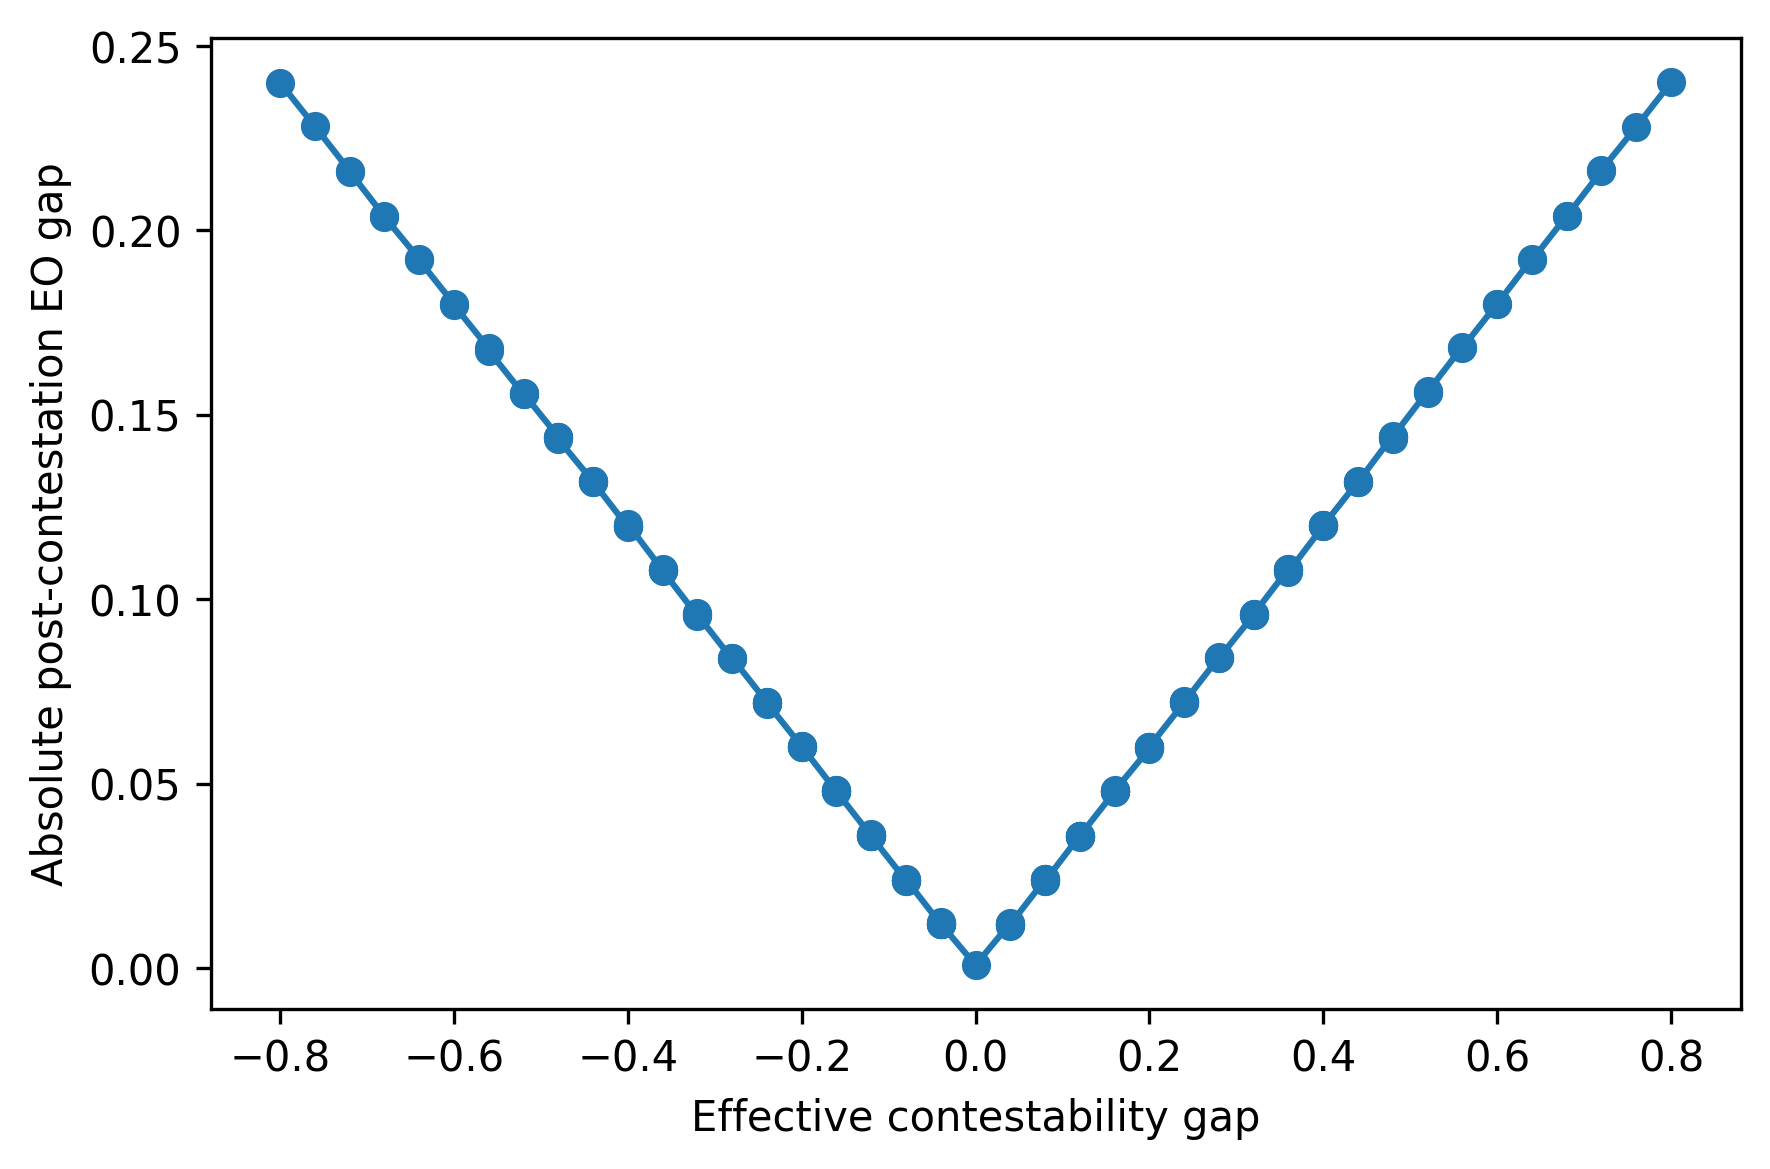
\includegraphics[width=.68\linewidth]{figures/FIG-01_contestability_gap.png}
\caption{Synthetic verification of the relationship between the effective
contestability difference and the absolute post-contestation
equal-opportunity gap $|\Delta'_{EO}|$.}
\Description{A V-shaped line plot showing the nonnegative absolute
post-contestation equal-opportunity gap against differences in effective
contestability.}
\label{fig:gap}
\end{figure}

\section{Formal symmetry and endogenous access}

Suppose an eligible individual appeals when perceived benefit $v$ exceeds net
cost $C_g-u_g$, where $u_g$ is continuous group-level assistance.  If $C_g$
has conditional CDF
$F_g$, then
\begin{equation}
 \alpha_g(u_g)=F_g(v+u_g).
 \label{eq:access}
\end{equation}
The same posted procedure or subsidy does not imply the same appeal
probability when cost distributions differ.  With common review success
$\rho$, effective correction is $\rho F_g(v+u_g)$.

If $F_a(x)>F_b(x)$ throughout the policy-relevant support and assistance must
be group blind, $u_a=u_b$, then equal effective access is unattainable in the
interior unless a boundary saturates both groups or another component of the
mechanism offsets the ordering.  This is a conditional impossibility result,
not a claim that equality is impossible under all policy designs.  Group-
specific assistance, changes to documentation requirements, review-quality
interventions, or saturation provide escape routes.

\begin{figure}[t]
\centering
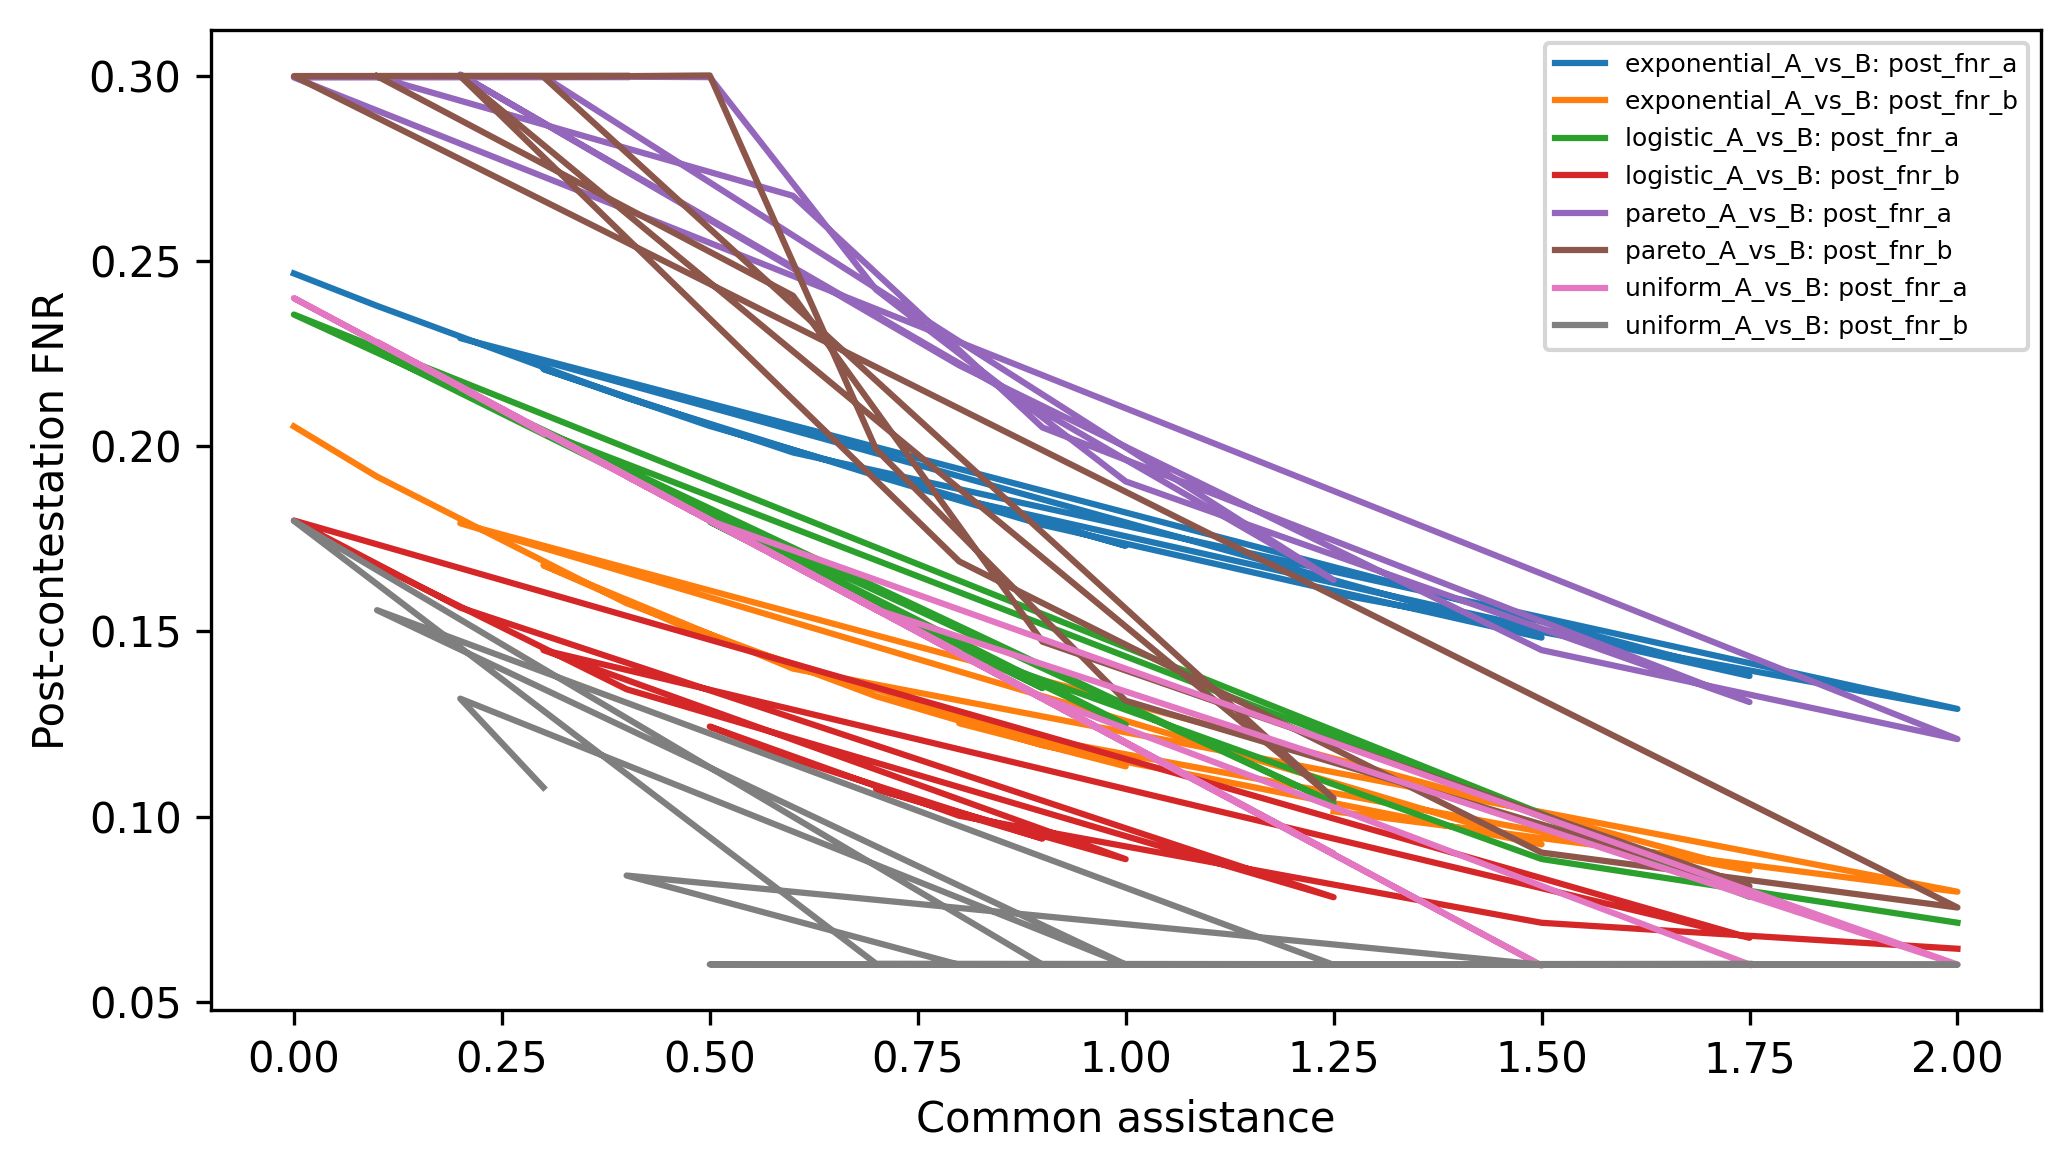
\includegraphics[width=.74\linewidth]{figures/FIG-02_equal_policy_heterogeneous_costs.png}
\caption{A formally equal assistance policy can produce unequal effective
access when groups face different appeal-cost distributions.}
\Description{Two appeal-access curves under the same assistance level; the
curves differ because the groups have different cost distributions.}
\label{fig:costs}
\end{figure}

\section{Allocating limited assistance}

Let $u_g\ge0$ be assistance to group $g$, $N_g$ its eligible population, and
$B$ a budget.  A planner may minimize aggregate final error plus a fairness
penalty,
\begin{equation}
 \min_u\quad L(u)+\lambda\Phi(u)
 \quad\text{s.t.}\quad \sum_g N_gu_g\le B,
 \label{eq:allocation}
\end{equation}
where appeal access follows Equation~\eqref{eq:access}.  For differentiable,
convex separable-welfare instances satisfying Slater's condition, with a
binding budget and an interior allocation, the KKT conditions equate weighted
marginal harm reduction per unit resource among assisted groups, adjusted by
the shadow price of budget.  A fairness-aware optimum can
therefore prioritize a group whose marginal disparity reduction is large even
when a purely accuracy-maximizing rule would not.

For indivisible interventions, the problem contains 0--1 knapsack as a
special case; this classical reduction motivates exact dynamic programming or
approximation rather than a claim of new complexity theory.  Our experiments
compare the fairness-aware rule with uniform, random, and proportional
baselines and expose the parameter $\lambda$ rather than silently fixing a
normative objective.

\begin{figure}[t]
\centering
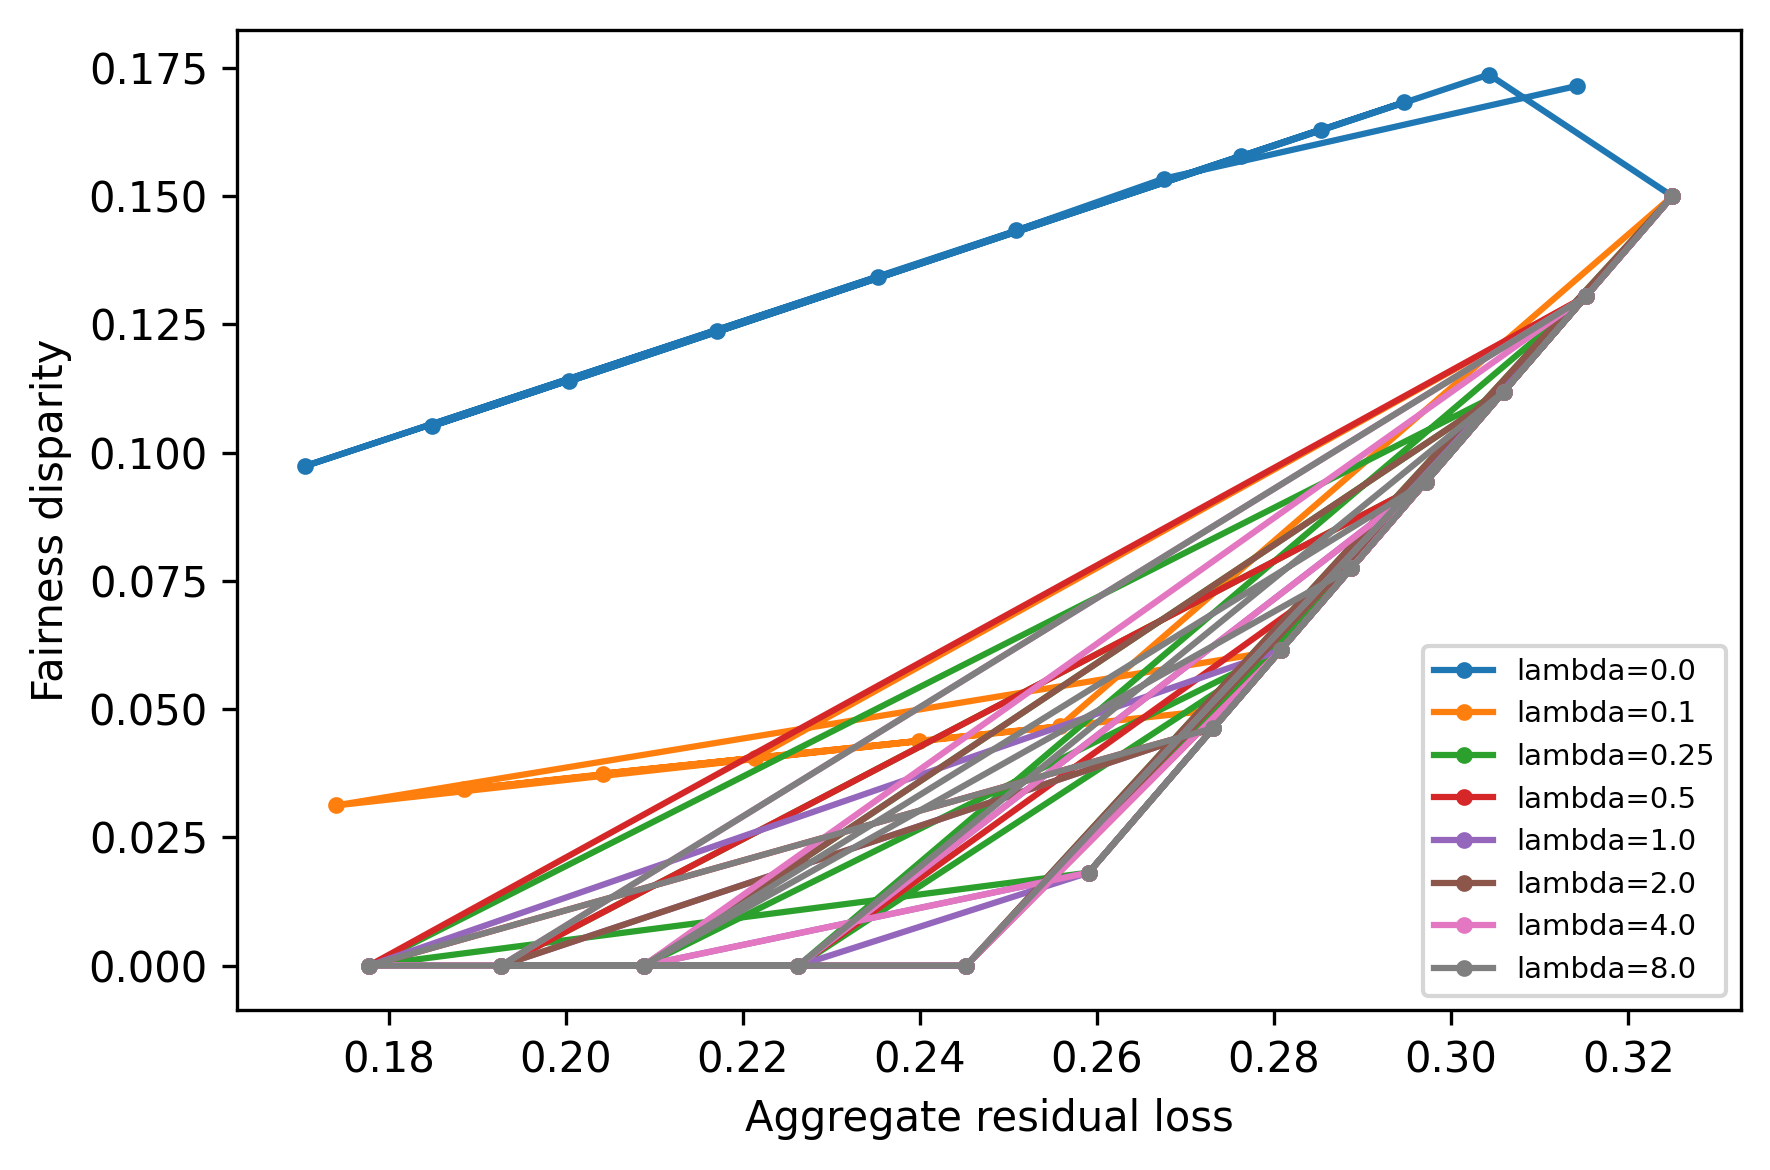
\includegraphics[width=.70\linewidth]{figures/FIG-03_fairness_utility_frontier.png}
\caption{The experimental fairness--utility frontier under limited
assistance.  The curve makes the normative trade-off explicit.}
\Description{A frontier plotting equal-opportunity disparity against aggregate
loss as the assistance allocation changes.}
\label{fig:frontier}
\end{figure}

\section{What appeal logs identify}

An ordinary log observes $G,D_0,A$ and the review outcome for appellants, but
typically not a valid $Y$ for non-appellants.  Let $d_g$ be the adverse-decision
mass, $a_g=\Prb(A=1\mid D_0=0,G=g)$, and let
$\eta_g=\Prb(Y=1\mid A=1,D_0=0,G=g)$ be the observed positive-label share
among appellants.  The latent positive share among non-appellants,
$q_g=\Prb(Y=1\mid A=0,D_0=0,G=g)$, can vary over $[0,1]$ without changing the
appeal-log distribution.
Hence the positive mass among adverse cases lies sharply in
\begin{equation}
 d_g\{a_g\eta_g+(1-a_g)q_g\},\qquad q_g\in[0,1].
\end{equation}
Combining this interval with the observed positive mass among initially
favorable cases yields sharp bounds on the group FNR.  Distinct worlds can
therefore have identical appeal logs but materially different oracle error
rates and fairness conclusions.

Representative random audits of adverse non-appellants identify $q_g$ under
valid labels and known inclusion probabilities.  Inverse-probability
estimation is then consistent, and uncertainty contracts with the effective
audit sample size.  Random auditing is a supporting design result familiar
from missing-data and selective-label settings; its importance here is that
it closes the precise gap left by self-selected appeal logs.

\begin{figure}[t]
\centering
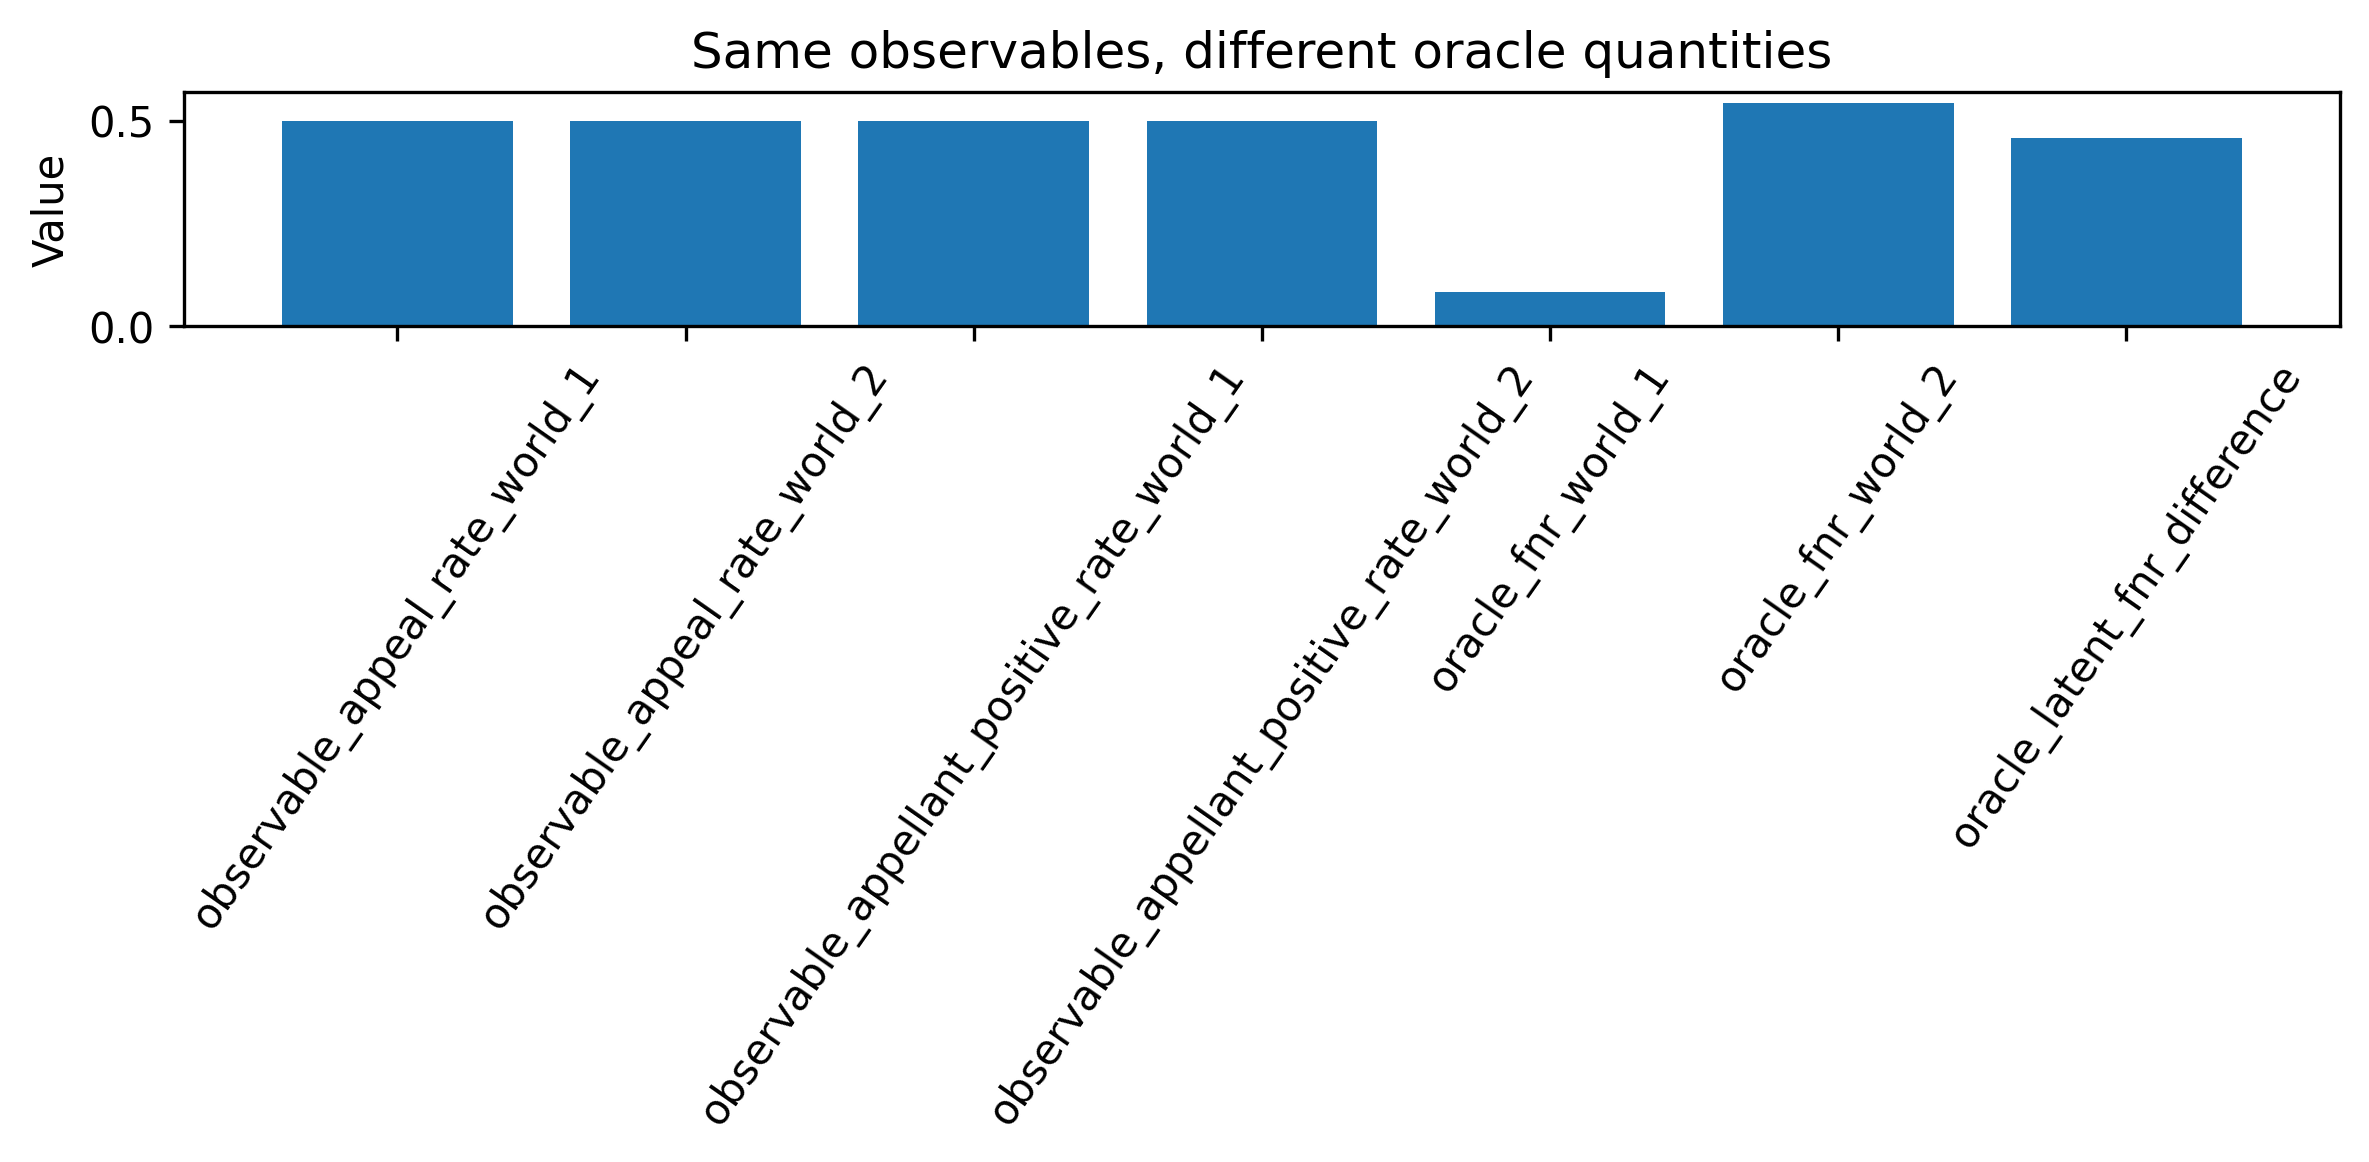
\includegraphics[width=.48\linewidth]{figures/FIG-04_observational_equivalence.png}
\hfill
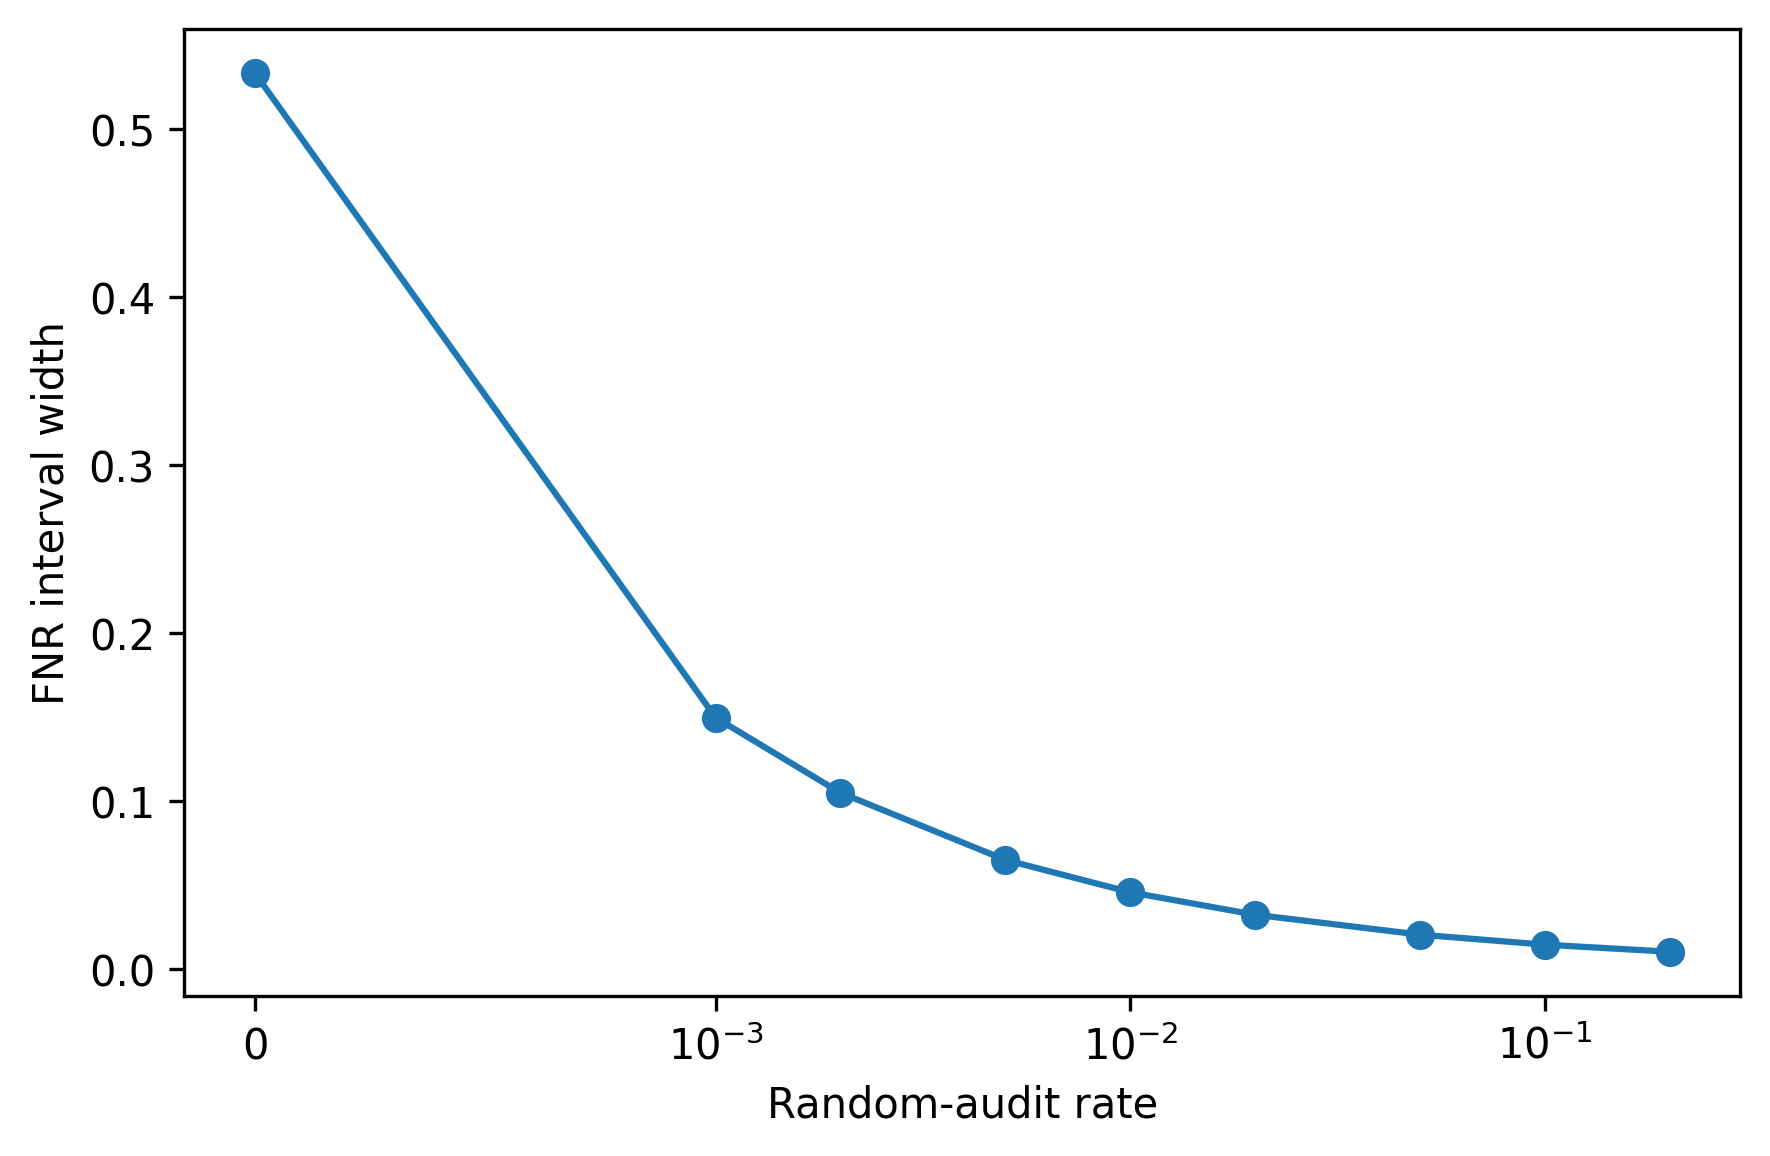
\includegraphics[width=.48\linewidth]{figures/FIG-05_audit_rate_interval_width.png}
\caption{Left: observationally equivalent appeal logs can conceal different
oracle FNRs. Right: representative auditing contracts the identified interval.}
\Description{The left panel compares latent worlds with identical observed
appeal logs but different false-negative rates. The right panel shows interval
width declining as the representative audit rate increases.}
\label{fig:id}
\end{figure}

\section{Experiments}

\subsection{Design}

The evaluation has six predeclared gates.  Unit and smoke tests precede the
scientific runs.  Synthetic experiments then test algebraic agreement,
interior-grid directional predictions, assistance allocation, observational
equivalence, sharp bounds, and audit-width contraction.  The final gate uses
Adult \citep{becker1996adult} and German Credit
\citep{hofmann1994german} as real classification tasks with a semisynthetic
post-decision mechanism.  Both are public UCI datasets distributed under
CC~BY~4.0.

For each real dataset we fit logistic regression, gradient boosting, and
random forest models.  Train, validation, and test partitions are separated;
group thresholds are calibrated on validation data and frozen before test
evaluation.  Five contestation regimes are fixed in advance: equal access and
moderate or strong advantage for either group.  Twenty paired seeds
(1729--1748) yield
$2\times3\times5\times20=600$ real-data runs.  We report two-sided 95\%
Student-$t$ intervals for paired seed-level pre/post changes.  These data do
not contain observed appeals, costs, or review behavior; only the prediction
task is empirical.

The complete pipeline contains 820 standardized seed-level CSV files: 220
synthetic/theorem files and 600 real-data files.  All commands returned zero,
and validation completed without errors or warnings.  The downloaded Kaggle
artifact is retained with a SHA-256 digest and an immutable extracted copy.

\begin{table}[t]
\centering
\caption{Computational environments and software used for development,
validation, and reproduction.  The phrase \emph{Not recorded} means that an
exact version was not recoverable from the authoritative archived artifacts.}
\label{tab:environment}
\footnotesize
\begin{tabularx}{\linewidth}{@{}p{.23\linewidth}YY@{}}
\toprule
Component & Authoritative final scientific run & Local development/reproduction \\
\midrule
\multicolumn{3}{@{}l}{\textit{A. Hardware and execution environment}}\\
Platform/OS & Kaggle Notebook; Linux (managed environment) & Windows (clean reproduction); ASUS TUF F15 hardware is author-reported \\
Accelerator & CPU only; Internet disabled & CPU execution; NVIDIA GeForce RTX 3050 (4 GB) present but not used in validated scientific runs \\
CPU & Model not exposed by archived Kaggle environment & Intel Core i5-12500H (author-reported) \\
RAM & Not exposed by archived Kaggle environment & 16 GB (author-reported) \\
Run record & ID 352782151; 2026-09-25 18:51:07--19:12:56 UTC & Clean reproduction of 220 synthetic/theorem outputs \\
\midrule
\multicolumn{3}{@{}l}{\textit{B. Software stack}}\\
Python & Not recorded & 3.11 \\
NumPy & Not recorded & 2.4.6 \\
pandas & Not recorded & 2.3.3 \\
SciPy & Not recorded & 1.17.1 \\
scikit-learn & Not recorded & 1.9.1 \\
Matplotlib & Not recorded & 3.11.2 \\
statsmodels & Not recorded & 0.15.0 \\
PyYAML & Not recorded & 6.0.3 \\
pytest & Not recorded & 8.4.2 \\
\bottomrule
\end{tabularx}
\end{table}

\subsection{Dataset and protocol data card}

Both prediction datasets are from the UCI Machine Learning Repository and are
distributed under CC~BY~4.0.  Adult combines the 32,561 training and 16,281
test records supplied by UCI; all 48,842 records remain after deterministic
schema conversion.  The target is income $>\$50{,}000$ (favorable $=1$;
$\le\$50{,}000$ unfavorable $=0$), and the protected attribute is sex coded
exactly as \texttt{Female}/\texttt{Male}.  German Credit contains 1,000 raw
and 1,000 prepared records.  UCI credit-risk label 1 (good) maps to favorable
1 and label 2 (bad) to 0.  Personal-status/sex codes A92 and A95 map to
\texttt{Female}; A91, A93, and A94 map to \texttt{Male}.  In both datasets the
group column is removed from classifier inputs.  German's source
personal-status/sex field is also removed.

Adult question marks are parsed as missing; German conversion introduces no
missing-value rule.  In the modeling pipeline, numeric missing values are
median-imputed and standardized; categorical missing values are
most-frequent-imputed and one-hot encoded with unknown levels ignored.  For
each seed, joint label--group stratification creates 60/20/20 percent
train/validation/test partitions: test uses seed $s$ and validation uses
$s+1$.  Logistic regression, histogram gradient boosting, and random forest
are fit on training data.  On validation data, each group's threshold is
selected from $\{0.01,\ldots,0.99\}$ to match the overall positive-class TPR
at threshold 0.5 as closely as possible; thresholds are then frozen on test.

The paired seed range is 1729--1748.  The five preregistered regimes set the
Female/Male values of $\alpha^+$ as follows: equal $(.50,.50)$; moderate
female $(.65,.35)$; strong female $(.75,.25)$; moderate male $(.35,.65)$; and
strong male $(.25,.75)$.  Every regime uses Female/Male values
$\alpha^-=(.25,.25)$, $\rho^+=(.80,.80)$, and $\rho^-=(.05,.05)$.  Dataset
features, targets, and initial predictions are empirical; appeal, review, and
final-decision variables are semisynthetic.

\subsection{Synthetic results}

The synthetic gates pass.  Across the EXP-01 grid, theoretical signed gaps
span $-0.24$ to $0.24$ and empirical means have absolute error between
$0.000441$ and $0.001621$.  EXP-02 covers signed gaps from $-0.15$ to $0.15$
with mean absolute error from $0.000640$ to $0.001522$.  The heterogeneous-
cost experiment has mean absolute errors from $0.000379$ to $0.001324$.

At interior budgets, the fairness-aware allocation produces a nontrivial
trade-off between the absolute equal-opportunity gap and aggregate loss.  On
the evaluated grid, it reduces the absolute gap relative to the evaluated
uniform, random, and proportional baselines.  In the
identification suite, four pairs of observationally equivalent worlds have
oracle FNR differences from $1/3$ to $2/3$.  Aggregate interval width falls
from $0.1496$ at audit rate $0.001$ to $0.0102$ at rate $0.20$, with reported
coverage 1.0 on the evaluated grid.

\subsection{Semisynthetic real-data results}

Table~\ref{tab:e6} gives the predeclared E6 decision.  On Adult, average
pre-contestation absolute equal-opportunity gaps range from 0.031 to 0.039.  Every one
of the 12 unequal-access model--scenario cells increases the absolute gap,
with all paired 95\% intervals excluding zero.  Mean increases range from
0.0442 to 0.1513.  All 12 signed shifts point toward the group with greater
false-denial access and exclude zero.

German Credit behaves differently.  Average initial gaps are 0.0275 for
random forest, 0.0742 for gradient boosting, and 0.0945 for logistic
regression.  The expected signed movement is resolved in 7 of 12 unequal-
access cells: 4/4 logistic, 3/4 gradient boosting, and 0/4 random forest.
Signed mean changes range from $-0.0700$ to $+0.0443$.  No German cell has a
paired interval supporting an increase in the absolute gap.  The signed
disparity often attenuates, crosses zero, or reverses, consistent with
Equation~\eqref{eq:signedgap}, while small test strata produce noisier
calibration and inference.

Overall accuracy improves with a positive paired interval in all 30 dataset--
model--scenario cells.  These German Credit results are consistent with the
signed-gap theory: review remains mostly corrective, while the fairness effect
may attenuate, cross, or reverse an existing disparity and is not
model-robust.  We classify E6 as a \emph{partial pass}.

\begin{table}[t]
\centering
\caption{Summary of unequal-access E6 cells. ``Signed resolved'' means the
paired 95\% interval excludes zero in the direction specified by the access
advantage.}
\label{tab:e6}
\begin{tabular}{lrrrr}
\toprule
Dataset & Cells & Signed resolved & Absolute increase & Accuracy increase\\
\midrule
Adult & 12 & 12 & 12 & 12\\
German Credit & 12 & 7 & 0 & 12\\
\bottomrule
\end{tabular}
\end{table}

\begin{figure}[t]
\centering
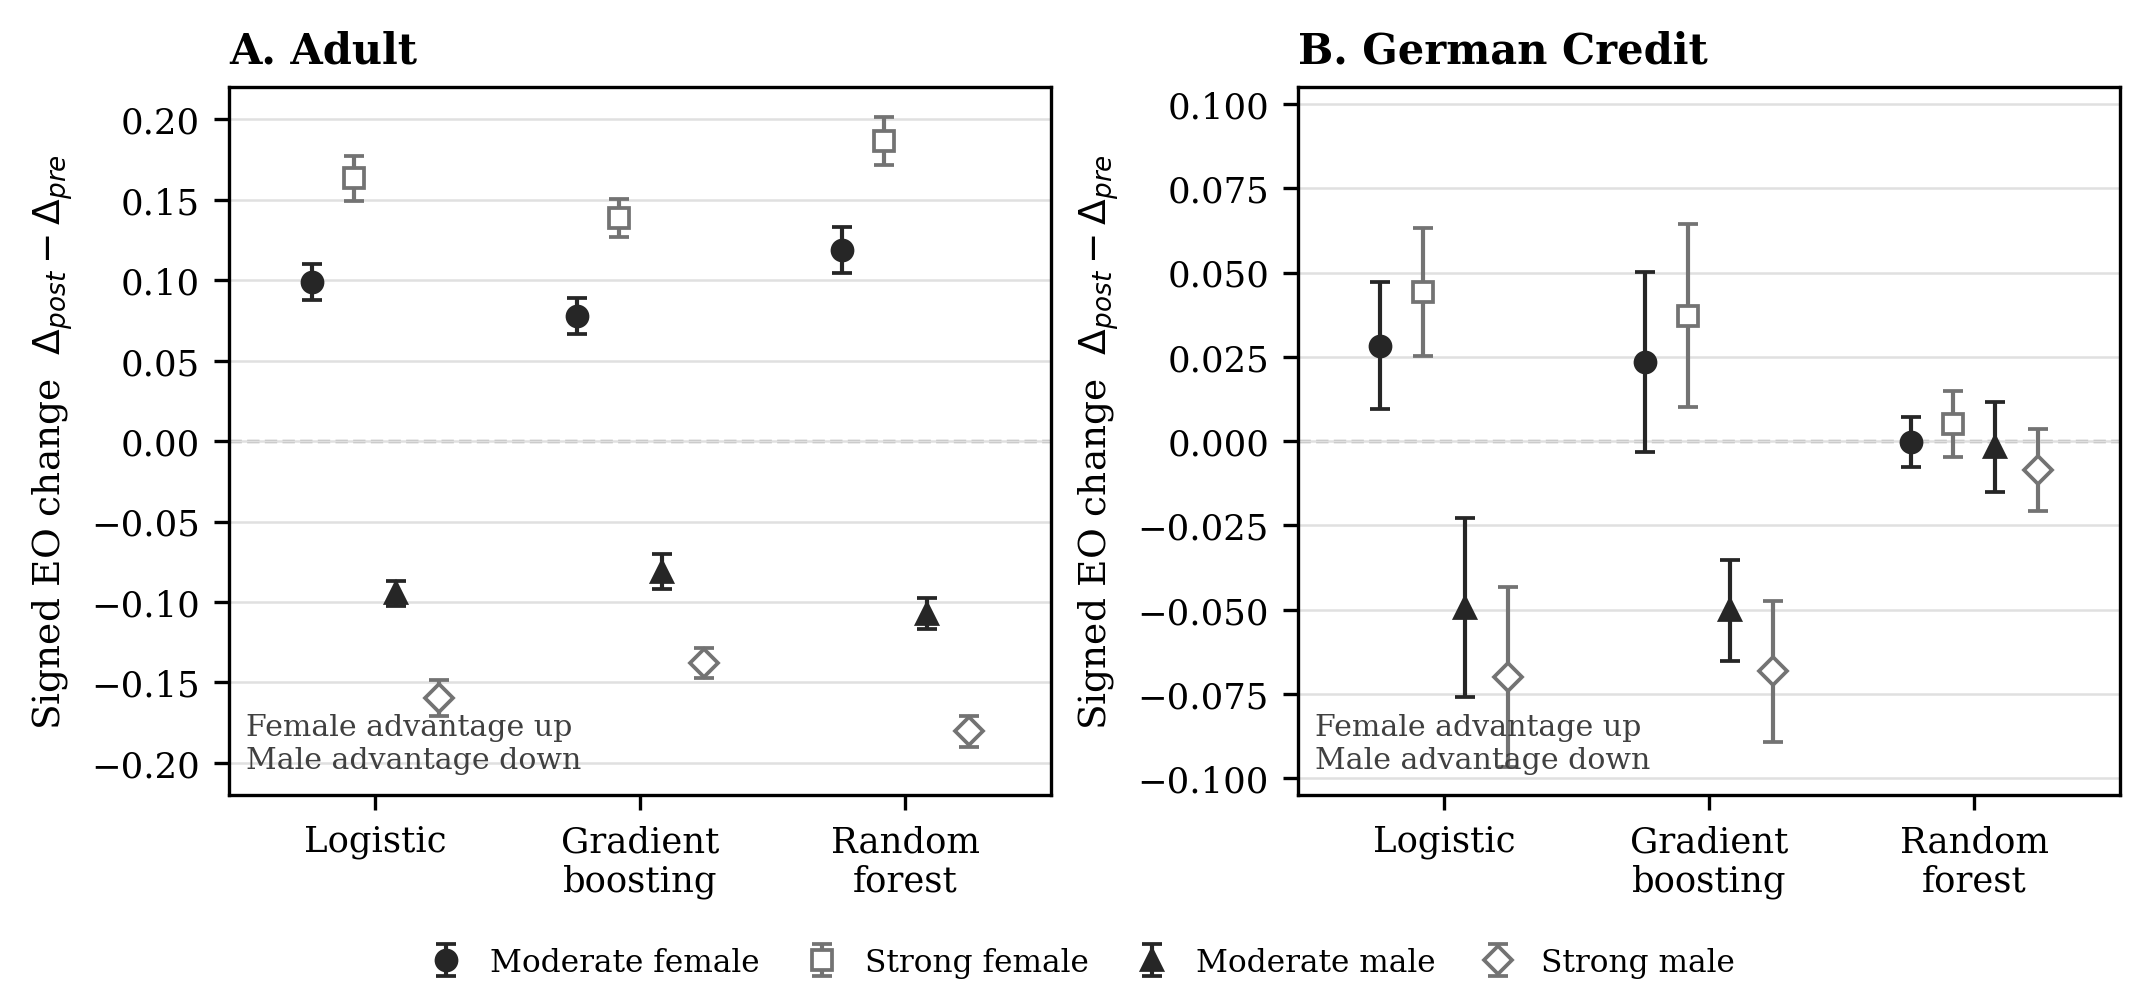
\includegraphics[width=.98\linewidth]{figures/FIG-05_signed_eo_change.png}
\caption{Paired change in the signed equal-opportunity disparity
$\Delta_{\mathrm{post}}-\Delta_{\mathrm{pre}}$ under the four unequal-access
regimes; bars are two-sided 95\% paired Student-$t$ intervals across 20 seeds.
The sign is Female minus Male, so female-advantage regimes move upward and
male-advantage regimes downward.  Adult resolves all 12 predicted directions;
German Credit resolves 7 of 12, and none for random forest.  Absolute-gap
changes are summarized in Table~\ref{tab:e6}: 12/12 positive on Adult and
0/12 positive on German Credit.}
\Description{Two-panel interval plot for Adult and German Credit. Each panel
shows signed equal-opportunity-gap changes for three classifiers and four
unequal-access regimes. Adult intervals consistently follow the access
advantage; German intervals are wider and random-forest intervals cross zero.}
\label{fig:real}
\end{figure}

\section{Discussion and limitations}

The main conceptual implication is that classifier fairness and final-decision
fairness are different estimands.  A system can become more accurate for every
group yet distribute corrections unequally.  Audits should record initial and
final decisions, appeal eligibility, attempted and completed appeals, review
outcomes, processing time, assistance, and representative labels among
non-appellants.  Reporting appeal success only among those who enter the
process is insufficient.

The theory does not rank fairness definitions or resolve normative trade-offs.
It assumes binary labels and decisions, a one-shot channel, stable review
behavior, and fixed groups.  It omits queues, deadlines, repeated appeals,
retaliation, classifier retraining, strategic institutions, and causal effects
of protected-group membership.  Reviewer accuracy can depend on case mix, so
expanding access may change $\rho$ rather than merely $\alpha$.  Assistance
may alter perceived benefit or evidentiary quality as well as cost.

Labels may be delayed, disputed, or affected by the decision.  Random audits
identify non-appellant outcomes only when selection is representative and
audit labels are valid.  Group-level equality can conceal intersectional and
within-group inequity.  The real-data component is semisynthetic and contains
no institutional estimates of appeal behavior or costs.  German Credit, in
particular, does not support a universal absolute-amplification claim.

The supplied novelty audit also limits the claim.  Contestability,
reviewability, procedural fairness, relative decision-set fairness, fair
recourse, heterogeneous appeal costs, human discretion, selective labels,
partial identification, random auditing, convex KKT conditions, and knapsack
structure are established topics.  The contribution is the specified
claimant-initiated correction mechanism and its exact fairness, identification,
and intervention consequences; no priority claim is made.

\section{Conclusion}

Post-decision review is not automatically a fairness safeguard.  Within the
specified claimant-initiated mechanism, exact transformation identities state
when equal opportunity, false-positive parity, equalized odds, or demographic
parity survive review.  The signed correction term can reinforce, attenuate,
cross, or reverse an existing disparity.  Endogenous participation explains
why formal symmetry can fail to produce effective symmetry; the same model
supports constrained assistance analysis and appeal-log-specific sharp bounds.
The evidence marks the empirical boundary honestly: consistent Adult effects,
partial directional support on German Credit, and no universal absolute-gap
amplification result.

\section*{Reproducibility statement}

The final audited Kaggle run is 352782151 (CPU; Internet disabled), executed
2026-09-25 18:51:07--19:12:56 UTC.  Its downloaded archive has SHA-256
\begin{center}
\small\texttt{AE30CA19BF912DB8FEB1BE33E263C994}\\[-2pt]
\texttt{F73ED3C2556E6EFF6D6EB69747BCBF1A}.
\end{center}
The analysis validates the exact factorial before computing paired intervals.
Configuration, seeds, standardized outputs, figures, gate decisions, and an
output-inventory regression test accompany the manuscript.

Code, configurations, and reproducibility artifacts are available at
\url{https://github.com/Ranjan-V/JAIR-Fairness-After-the-Decision}.
The source code is released under the MIT License, and author-generated
research artifacts are released under CC BY 4.0. Third-party datasets retain
their original source terms and are not redistributed in the repository.

A fresh clean-environment reproduction regenerated all 220 synthetic/theorem
outputs.  All 220 matched the archived numerical content at absolute and
relative tolerance $10^{-6}$; the maximum absolute numerical difference was
$5.39\times10^{-8}$.  This is a scientific-content reproduction, not a claim
of byte equality.  Cross-platform line endings, serialized parameter keys,
and final optimizer digits differ across the audited Linux and Windows
environments; these differences are documented in the reproduction audit.

\appendix
\section{Technical Appendix: Proofs and Boundary Cases}
\label{app:proofs}

This appendix states the exact scope of every named mathematical result used
by the paper.  Conditional probabilities are asserted only when their
conditioning events have positive probability.  All one-sided results assume
that only an adverse initial decision can change and that a non-appellant
retains the initial decision.

\subsection{Operators and confusion-rate transformations}

\paragraph{Theorem 1 (linear operator preservation criterion).}
Let $V$ be a finite-dimensional vector space of feasible signed
perturbations, let $T_K:V\to V$ be the linear map induced by a fixed
collection of stochastic kernels, and let $L:V\to W$ encode a homogeneous
linear fairness constraint.  The following are equivalent:
\begin{enumerate}
  \item $Lv=0$ implies $LT_Kv=0$ for every $v\in V$;
  \item $\ker L\subseteq\ker(LT_K)$;
  \item there is a linear map $M:\operatorname{im}L\to W$ such that
        $LT_K=ML$ on $V$.
\end{enumerate}

\begin{proof}
The first two conditions are identical.  Under the second, define
$M(Lv)=LT_Kv$.  If $Lv=Lw$, then $v-w\in\ker L$, so
$LT_K(v-w)=0$ and the definition does not depend on the representative.
It is linear by construction.  Conversely, $LT_K=ML$ immediately implies
$LT_Kv=0$ whenever $Lv=0$.
\end{proof}

For probability models, $V$ must be the span of feasible signed differences.
An assertion made only on a thin or boundary-only subset of probability
vectors does not automatically extend to the full algebraic kernel.  Affine
constraints must be homogenized with a constant coordinate.

\paragraph{Proposition 1 (one-sided confusion-rate transformation).}
For every group $g$ with defined label-conditional rates,
\begin{align*}
 \mathrm{TPR}'_g&=\mathrm{TPR}_g+\mathrm{FNR}_g\kappa_g^+,&
 \mathrm{FNR}'_g&=\mathrm{FNR}_g(1-\kappa_g^+),\\
 \mathrm{FPR}'_g&=\mathrm{FPR}_g+\mathrm{TNR}_g\kappa_g^-,&
 \mathrm{TNR}'_g&=\mathrm{TNR}_g(1-\kappa_g^-).
\end{align*}

\begin{proof}
Conditional on $Y=1,G=g$, a final positive is either an initial positive or
an initial negative followed by appeal and reversal.  These events are
disjoint, and the latter has probability
$\mathrm{FNR}_g\alpha_g^+\rho_g^+=\mathrm{FNR}_g\kappa_g^+$.
Complementation gives the FNR identity.  Repeating the argument in the
$Y=0$ stratum gives FPR and TNR.
\end{proof}

\paragraph{Corollary 1 (positive-decision rate).}
With $\pi_g=\Prb(Y=1\mid G=g)$ and
$r_g=\Prb(D_0=1\mid G=g)$,
\[
r'_g=r_g+\pi_g\mathrm{FNR}_g\kappa_g^+
 +(1-\pi_g)\mathrm{TNR}_g\kappa_g^-.
\]

\begin{proof}
Condition on $Y$ and substitute Proposition 1.
\end{proof}

\paragraph{Proposition 2 (two-sided transformation).}
If $q_g^y=\Prb(D_1=0\mid D_0=1,Y=y,G=g)$, then
\[
 \mathrm{TPR}'_g=t_g(1-q_g^1)+(1-t_g)\kappa_g^+,
 \qquad
 \mathrm{FPR}'_g=f_g(1-q_g^0)+(1-f_g)\kappa_g^-.
\]

\begin{proof}
Partition on $D_0$ within each label stratum and apply the two rows of the
transition kernel.
\end{proof}

\subsection{Fairness preservation and signed disparity}

\paragraph{Theorem 2 (equal-opportunity preservation).}
If $t_A=t_B=t$, then post-contestation equal opportunity holds if and only if
$(1-t)(\kappa_A^+-\kappa_B^+)=0$.  When $t<1$, this is equivalent to
$\kappa_A^+=\kappa_B^+$; when $t=1$, it is automatic.

\begin{proof}
Subtract the two TPR identities in Proposition 1.
\end{proof}

\paragraph{Theorem 3 (FPR-parity preservation).}
If $f_A=f_B=f$, then post-contestation FPR parity holds if and only if
$(1-f)(\kappa_A^--\kappa_B^-)=0$.

\begin{proof}
Subtract the two FPR identities in Proposition 1.
\end{proof}

\paragraph{Corollary 2 (equalized odds).}
Under initial equalized odds, final equalized odds holds exactly when both
conditions in Theorems 2 and 3 hold.

\begin{proof}
Equalized odds is the conjunction of equal TPR and equal FPR.
\end{proof}

\paragraph{Theorem 4 (demographic-parity preservation).}
If $r_A=r_B$ initially, demographic parity is preserved exactly when
\[
\pi_A\mathrm{FNR}_A\kappa_A^+
 +(1-\pi_A)\mathrm{TNR}_A\kappa_A^-
=\pi_B\mathrm{FNR}_B\kappa_B^+
 +(1-\pi_B)\mathrm{TNR}_B\kappa_B^-.
\]

\begin{proof}
Subtract the two identities in Corollary 1 and use $r_A-r_B=0$.
\end{proof}

\paragraph{Proposition 3 (universal one-sided preservation).}
At a fixed common initial TPR $t<1$, a pair of one-sided operators preserves
equal opportunity for every admissible group distribution if and only if the
two $Y=1$ adverse-to-positive transition probabilities agree.  The analogous
claim holds for FPR at a common $f<1$.

\begin{proof}
Sufficiency follows from Theorem 2.  Necessity follows because the multiplier
$1-t$ (or $1-f$) is strictly positive.
\end{proof}

\paragraph{Theorem 5 (exact signed-gap dynamics).}
Let $d=t_A-t_B$ and
$c=(1-t_A)\kappa_A^+-(1-t_B)\kappa_B^+$.  Then $d'=d+c$ and
\begin{align*}
|d'|>|d|&\iff c(2d+c)>0,\\
|d'|<|d|&\iff c(2d+c)<0,\\
|d'|=|d|&\iff c=0\ \text{or}\ c=-2d.
\end{align*}
Direction reverses exactly when $d(d+c)<0$, and final equality holds exactly
when $c=-d$.

\begin{proof}
The identity $d'=d+c$ follows from Proposition 1.  Since absolute gaps are
nonnegative,
$|d+c|^2-|d|^2=c(2d+c)$ has the same sign as their difference.  The remaining
claims follow directly from the signs of $d,d+c$ and from $d+c=0$.
\end{proof}

\paragraph{Theorem 6 (tight attainable bounds).}
For unrestricted independent $\kappa_A^+,\kappa_B^+\in[0,1]$,
\[
d'\in[t_A-1,1-t_B].
\]
The minimum attainable absolute gap is zero when this interval contains zero
and otherwise is the distance from the interval to zero; the maximum is the
larger absolute endpoint.

\begin{proof}
Writing $a=1-t_A$ and $b=1-t_B$, the correction $a\kappa_A^+-b\kappa_B^+$
ranges continuously over $[-b,a]$.  Adding $d$ gives the displayed interval.
The absolute-value extrema follow from elementary interval geometry and are
attained at a corner or a feasible root.
\end{proof}

\paragraph{Corollary 3 (initially fair case).}
If $t_A=t_B=t$, then
$|d'|=(1-t)|\kappa_A^+-\kappa_B^+|\le1-t$, and the bound is tight.

\subsection{Endogenous access and the conditional impossibility}

\paragraph{Proposition 4 (threshold appeal response).}
If perceived value is deterministic at $v_g^y$ and the conditional cost CDF
is $F_g^y$, then $\alpha_g^y(u)=F_g^y(v_g^y+u)$.  For random value $V$,
\[
\alpha_g^y(u)=
\E\!\left[F_{C\mid V,g,y}(V+u\mid V,G=g,Y=y,D_0=0)\right].
\]

\begin{proof}
The appeal event is $\{C\le V+u\}$.  Condition on the declared stratum and,
in the random-value case, condition once more on $V$.
\end{proof}

\paragraph{Proposition 5.} \emph{Comparative statics.}
The appeal response is nondecreasing and right-continuous in assistance.  If
the conditional cost law has density $f_{C\mid V,g,y}$ and differentiation
under the expectation is valid, then
\[
(\alpha_g^y)'(u)=
\E[f_{C\mid V,g,y}(V+u\mid V,g,y)]\ge0.
\]

\begin{proof}
The indicator of $C\le V+u$ is pointwise nondecreasing in $u$, and its
expectation is a shifted CDF mixture.  Right-continuity follows from CDF
right-continuity and bounded convergence.  Under the stated regularity,
differentiation under the expectation yields the density formula.
\end{proof}

\paragraph{Theorem 7 (formal symmetry versus effective equality).}
Under common assistance $u$, deterministic perceived value $v$, and common
review success $\rho>0$,
\[
\kappa_A^+(u)-\kappa_B^+(u)
=\rho\{F_A^+(v+u)-F_B^+(v+u)\}.
\]
Thus effective correction parity holds exactly when the two conditional CDFs
agree at the operative threshold.

\begin{proof}
Apply Proposition 4 and multiply each appeal probability by the common
review-success rate.
\end{proof}

\paragraph{Theorem 8 (group-blind policy impossibility).}
Assume initial $t_A=t_B=t<1$, group-blind $u$ in a feasible set $U$, common
$v$, common $\rho>0$, and
$F_A^+(v+u)<F_B^+(v+u)$ for every $u\in U$.  No feasible group-blind policy
preserves equal opportunity.

\begin{proof}
Theorem 7 gives $\kappa_A^+(u)<\kappa_B^+(u)$.  Theorem 2 then gives
\[
t'_A-t'_B=(1-t)\rho\{F_A^+(v+u)-F_B^+(v+u)\}<0.
\]
The strictness assumptions are essential: saturation, a crossing point,
zero review success, a perfect initial classifier, unequal review quality, or
group-specific assistance can each invalidate the conclusion.
\end{proof}

\subsection{Limited-resource allocation}

Define $\mathcal{R}_g(u_g)=
\mathrm{FNR}_g[1-\rho_g^+\alpha_g^+(u_g)]$.

\paragraph{Theorem 9 (existence).}
On a nonempty compact product domain, if every $\mathcal{R}_g$ and resource cost $c_g$
is continuous and the budget set is nonempty, both the minimax residual-risk
program and the stated welfare-plus-disparity program attain optima.

\begin{proof}
The budget sublevel set is closed in a compact domain, hence compact.  Finite
maxima, sums, and absolute differences of continuous functions are continuous.
Weierstrass' theorem gives attainment.
\end{proof}

\paragraph{Theorem 10 (convexity conditions).}
If every appeal response is concave, each cost is convex, and the domain is
convex, then every $\mathcal{R}_g$ is convex and the minimax problem is convex in
epigraph form.  The separable welfare objective is convex.  A disparity-
penalized objective is convex only when its pairwise absolute residual-risk
differences are convex (for example, under affine residual risks).

\begin{proof}
$\mathcal{R}_g$ is a constant plus a nonpositive multiple of a concave response, hence
convex.  Finite maxima preserve convexity, and convex cost sublevel sets are
convex.  Weighted sums preserve convexity.  The final qualification is needed
because an absolute difference of two general convex functions need not be
convex.
\end{proof}

\paragraph{Theorem 11 (KKT marginal rule).}
For the differentiable convex separable-welfare program under Slater's
condition, there are nonnegative multipliers $\eta,\ell_g,h_g$ satisfying
\[
w_g\mathcal{R}'_g(u_g)+\eta c'_g(u_g)-\ell_g+h_g=0
\]
and complementary slackness.  If the budget binds,
$0<u_g<\bar u_g$, and $c'_g(u_g)>0$, then
\[
-\frac{w_g\mathcal{R}'_g(u_g)}{c'_g(u_g)}=\eta.
\]

\begin{proof}
Under convexity and Slater's condition, KKT conditions are necessary and
sufficient.  Interior box constraints set $\ell_g=h_g=0$; division by the
positive marginal resource cost gives the displayed equality.  Boundary
groups obey inequalities rather than this equality.
\end{proof}

\paragraph{Proposition 6 (minimum budget for a target).}
If each $\mathcal{R}_g$ is continuous and strictly decreasing over its effective range
and each $c_g$ is nondecreasing, define
$u_g^{\min}(\epsilon)=\inf\{u:\mathcal{R}_g(u)\le\epsilon\}$.  The common target is
feasible exactly when every set is nonempty and
$B\ge\sum_gc_g(u_g^{\min})$.

\begin{proof}
Continuity makes each nonempty target sublevel closed, so the infimum is
attained.  Strict monotonicity makes every feasible component at least its
minimum.  Nondecreasing costs make the sum a necessary budget; choosing the
componentwise minima proves sufficiency.
\end{proof}

For $\mathrm{FNR}_g>0$ and $\rho_g>0$, the untruncated required appeal
probability is
$p_g^*=(1-\epsilon/\mathrm{FNR}_g)/\rho_g$.  If $p_g^*>1$, equivalently
$\epsilon<\mathrm{FNR}_g(1-\rho_g)$, the target is infeasible even with
universal appeal.  This boundary must not be hidden by clipping $p_g^*$.

\paragraph{Theorem 12 (discrete allocation complexity).}
With binary-encoded nonnegative integer intervention costs and benefits, the
threshold decision version of welfare-maximizing indivisible assistance is
weakly NP-complete, even for one group.

\begin{proof}
Map an arbitrary 0--1 knapsack instance identically to individuals with the
same costs and encoded expected benefits, the same budget, and the same target
benefit.  Feasible subsets and objective values coincide.  Membership in NP
follows by checking a proposed subset.  The inherited hardness is weak, not
strong.
\end{proof}

\subsection{Identification and statistical auditing}

\paragraph{Theorem 13 (appeal-log non-identification).}
Without restrictions on appeal selection, ordinary appeal logs do not identify
the final FNR even with perfect review and observed appellant labels.

\begin{proof}
Let every case have $D_0=0$, fix
$\Prb(A=1)=a\in(0,1)$ and
$\Prb(Y=1\mid A=1)=p\in(0,1)$, and let perfect review set $D_1=Y$ for
appellants.  Non-appellants keep $D_1=0$.  Vary
$q=\Prb(Y=1\mid A=0)$ over $[0,1]$.  Since $Y$ is unobserved exactly in
the non-appellant stratum, all values of $q$ yield the same observed law, but
\[
\mathrm{FNR}'(q)=\frac{(1-a)q}{ap+(1-a)q}
\]
is strictly increasing in $q$.
\end{proof}

\paragraph{Corollary 5 (fairness non-identification).}
Applying Theorem 13 separately to two groups gives observationally equivalent
joint laws with different signed and absolute equal-opportunity gaps.  With
positive fixed appellant-positive mass, a unit gap is approached but not
attained.

\paragraph{Theorem 14 (sharp no-assumption FNR bounds).}
Let
$s=\Prb(D_0=1,Y=1\mid g)$,
$m=\Prb(D_0=0,A=1,Y=1\mid g)$,
$n=\Prb(D_0=0,A=0\mid g)$,
let $\rho$ be the identified mean reversal probability among appealed
positives, and let $z\in[0,n]$ be the latent positive mass among adverse
non-appellants.  Then
\[
F(z)=\frac{m(1-\rho)+z}{s+m+z}.
\]
When $s+m>0$ and $s+\rho m>0$, its sharp identified set is
\[
\left[\frac{m(1-\rho)}{s+m},
\frac{m(1-\rho)+n}{s+m+n}\right].
\]
If $s+m>0$ but $s+\rho m=0$, the set is $\{1\}$.  If
$s=m=0<n$, the set over compatible laws with a nonempty positive stratum is
also $\{1\}$; if $s=m=n=0$, the FNR is undefined under every compatible law.

\begin{proof}
Where defined,
\[
F'(z)=\frac{s+\rho m}{(s+m+z)^2}\ge0.
\]
Endpoint substitution gives the first interval.  The stated boundary cases
follow by direct substitution.  Sharpness holds because every feasible $z$
can be assigned inside the unobserved stratum without changing the observed
law.
\end{proof}

\paragraph{Proposition 7 (propensity-restricted sharp bounds).}
Assume $m>0$ and
$0<\underline\alpha\le\alpha\le\overline\alpha\le1$, where
$\alpha=m/(m+z)$.  Then
\[
z\in\left[
m\frac{1-\overline\alpha}{\overline\alpha},
m\frac{1-\underline\alpha}{\underline\alpha}
\right]\cap[0,n].
\]
Substitution into $F(z)$ gives sharp restricted bounds.

\begin{proof}
Solve $\alpha=m/(m+z)$ for $z=m(1-\alpha)/\alpha$.  This map is decreasing
on $(0,1]$, which reverses the two propensity endpoints.  Intersecting with
the feasible mass interval is necessary and sufficient.  If the intersection
is empty, the restriction is falsified by the observed masses.
\end{proof}

\paragraph{Theorem 15 (identification by representative audits).}
If each adverse non-appellant is audited with positive probability independently
of $Y$ conditional on the recorded stratum, and the audit reveals $Y$ without
error, then the missing prevalence $q$ and hence $z=nq$, the final FNR, and
post-contestation disparities are identified.

\begin{proof}
Conditional independence gives
\[
\Prb(Y=1\mid \text{audit}=1,D_0=0,A=0,G=g)
=\Prb(Y=1\mid D_0=0,A=0,G=g)=q_g.
\]
All remaining terms in Theorem 14 are observed.
\end{proof}

\paragraph{Proposition 8 (finite-audit contraction).}
For $M_g\ge1$ independently audited non-appellants and positive fraction
$\widehat q_g$, Hoeffding's inequality gives, with probability at least
$1-\delta$,
\[
|\widehat q_g-q_g|\le
e_g=\sqrt{\frac{\log(2/\delta)}{2M_g}}.
\]
After clipping the prevalence interval to $[0,1]$ and propagating it through
$F(n_gq)$, its width is at most
\[
\frac{2n_g(s_g+\rho_gm_g)}{(s_g+m_g)^2}e_g
\]
when $s_g+m_g>0$.

\begin{proof}
Hoeffding gives the prevalence event.  Theorem 14's map is monotone, so its
image is a confidence interval.  Its derivative with respect to $q$ is
$n_g(s_g+\rho_gm_g)/(s_g+m_g+n_gq)^2$, bounded above by the displayed
coefficient without $2e_g$.  The mean-value theorem completes the bound.
\end{proof}

\paragraph{Proposition 9 (simultaneous group bounds).}
For $K$ groups, setting
\[
e_g=\sqrt{\frac{\log(2K/\delta)}{2M_g}}
\]
gives simultaneous coverage at least $1-\delta$ for all group prevalences,
FNR images, and interval-derived pairwise gaps.

\begin{proof}
Apply Hoeffding at error probability $\delta/K$ within each group and take a
union bound.  Monotone image and interval arithmetic preserve the joint
coverage event.
\end{proof}

\subsection{Audit disposition and code correspondence}

The proof audit found no contradiction in the central signed-gap,
preservation, endogenous-access, allocation, or non-identification results.
It did require three substantive clarifications: Theorem 1 is now stated on a
signed-perturbation space rather than inferred from an unspecified probability
domain; Proposition 6 exposes infeasible targets instead of clipping the
required appeal probability; and Theorem 14/Proposition 7 now handle zero-mass
boundaries explicitly.  Regression tests cover the new identification
boundaries.  The theorem-to-code correspondence remains diagnostic rather
than a substitute for proof.


\printbibliography

\section{Reproducibility Checklist for JAIR}

The answers below use the checklist distributed in the official JAIR author
kit downloaded on 27 September 2026.

\subsection*{All articles}

\begin{enumerate}
  \item All claims investigated in this work are clearly stated. \textbf{Yes.}
  \item Clear explanations are given of how the work substantiates the claims.
    \textbf{Yes.}
  \item Limitations or technical assumptions are stated clearly and
    explicitly. \textbf{Yes.}
  \item Conceptual outlines or pseudocode descriptions of introduced AI
    methods and important implementation details are provided.
    \textbf{Yes.} The mathematical operators, optimization problems, data
    protocol, and executable implementation details accompany the submission.
  \item Motivation is provided for design choices, parameters, datasets, and
    protocols beyond metrics. \textbf{Yes.}
\end{enumerate}

\subsection*{Articles containing theoretical contributions}

Does this paper make theoretical contributions? \textbf{Yes.}

\begin{enumerate}
  \item All assumptions and restrictions are stated clearly and formally.
    \textbf{Yes.}
  \item All novel claims are stated formally. \textbf{Yes.}
  \item Proofs of all non-trivial claims are provided in sufficient detail for
    verification by readers with relevant expertise. \textbf{Yes.}
  \item Complex formalism is motivated and explained clearly. \textbf{Yes.}
  \item Mathematical notation enhances clarity and gratuitous formalism is
    avoided. \textbf{Yes.}
  \item Appropriate citations are given for non-trivial theoretical tools and
    techniques. \textbf{Yes.}
\end{enumerate}

\subsection*{Articles reporting computational experiments}

Does this paper include computational experiments? \textbf{Yes.}

\begin{enumerate}
  \item All required source code is included in an appendix or will be made
    publicly available upon publication. \textbf{Yes.} The complete code is
    publicly available at
    \url{https://github.com/Ranjan-V/JAIR-Fairness-After-the-Decision}.
  \item The source code has a license permitting reproducibility use.
    \textbf{Yes.} Author-written source code is licensed under the MIT License.
  \item The source code has a license permitting general research use.
    \textbf{Yes.} Author-written source code is licensed under the MIT License.
  \item Raw, unaggregated experimental data is included or will be publicly
    available upon publication. \textbf{Yes.} All 820 standardized seed-level
    experimental output files are included in the public repository. Raw
    third-party UCI datasets are excluded and must be obtained from source.
  \item The unaggregated data has a license permitting reproducibility use.
    \textbf{Yes.} Author-generated experimental outputs are licensed under
    CC~BY~4.0; third-party datasets retain their original UCI source terms.
  \item The unaggregated data has a license permitting general research use.
    \textbf{Yes,} under the same license distinction.
  \item Random-number generation and seeds are described sufficiently for
    replication. \textbf{Yes.}
  \item The execution environment, hardware, operating system, and software
    versions are described. \textbf{Partially.} The CPU-only Kaggle setting,
    exact dependency constraints, and clean-environment versions are recorded;
    the managed worker's CPU model and RAM were not exposed in the archive.
  \item Evaluation metrics are explained and motivated. \textbf{Yes.}
  \item The number of algorithm runs is reported. \textbf{Yes.}
  \item Unsuccessful or unsatisfactory experiments have not been silently
    omitted. \textbf{Yes.}
  \item Results include variation, confidence, or other distributional
    information beyond point summaries. \textbf{Yes.}
  \item All algorithm and hyperparameter settings and their selection method
    are reported. \textbf{Yes.}
  \item The range and number of settings explored before the final experiments
    and optimization effort are indicated. \textbf{Partially.} The
    predeclared final factorial and thresholds are archived; this study did not
    conduct a broad hyperparameter search.
  \item Appropriate statistical hypothesis tests are used in the presence of
    noise. \textbf{Yes.} Paired two-sided 95\% Student-$t$ intervals are used
    for seed-level changes; conclusions are stated as interval resolutions,
    not as universal population claims.
\end{enumerate}

\subsection*{Articles using datasets}

Does this work rely on one or more datasets? \textbf{Yes.}

\begin{enumerate}
  \item Newly introduced datasets are included or will be public with a
    research-use license. \textbf{Not applicable.} No new dataset is
    introduced.
  \item A newly introduced dataset has a reproducibility-use license.
    \textbf{Not applicable.}
  \item A newly introduced dataset has a general research-use license.
    \textbf{Not applicable.}
  \item Datasets from public sources have appropriate citations.
    \textbf{Yes.}
  \item Datasets from the literature are publicly available.
    \textbf{Yes.}
  \item New or non-public datasets are described in detail.
    \textbf{Not applicable.}
  \item Preprocessing and splitting methods are described in detail.
    \textbf{Yes.} The manuscript data card records source and prepared counts,
    label and group mappings, feature exclusion, missing-value handling,
    encoding, scaling, splitting, threshold calibration, models, seeds, and
    every semisynthetic contestation parameter; executable preprocessing is
    supplied.
\end{enumerate}


\end{document}
